\documentclass[10.5pt,a4paper]{article}
\usepackage[margin=18mm,top=16mm,bottom=18mm]{geometry}
\usepackage{amsmath,amssymb}
\usepackage{graphicx}
\usepackage{booktabs}
\usepackage{tabularx}
\usepackage{array}
\usepackage{enumitem}
\usepackage{natbib}
\usepackage[hidelinks]{hyperref}
\usepackage{microtype}
\usepackage[T1]{fontenc}
\usepackage[utf8]{inputenc}
\usepackage{lmodern}
\usepackage{xcolor}
\usepackage{titlesec}
\usepackage{tcolorbox}
\usepackage{caption}

\captionsetup{font=footnotesize,labelfont=bf,skip=3pt}

% Compact section styling
\titleformat{\section}[hang]{\normalfont\large\bfseries}{\thesection.\ }{0pt}{}
\titlespacing*{\section}{0pt}{6pt}{2pt}
\titleformat{\subsection}[hang]{\normalfont\normalsize\bfseries}{\thesubsection\ }{0pt}{}
\titlespacing*{\subsection}{0pt}{4pt}{2pt}
\titleformat{\subsubsection}[hang]{\normalfont\small\bfseries}{\thesubsubsection\ }{0pt}{}
\titlespacing*{\subsubsection}{0pt}{3pt}{1pt}

\graphicspath{{figures/}}
\setlength{\parindent}{0pt}
\setlength{\parskip}{0.28em}
\setlength{\emergencystretch}{2em}

% Custom table column types
\newcolumntype{L}[1]{>{\raggedright\arraybackslash}p{#1}}
\newcolumntype{C}[1]{>{\centering\arraybackslash}p{#1}}
\newcolumntype{R}[1]{>{\raggedleft\arraybackslash}p{#1}}

\begin{document}

% Compact Title Block
\begin{center}
  {\Large\textbf{Application of Built-in Adaptive Remeshing and Mesh Refinement Features in Abaqus to Fracture Simulations Using Phase-field User Elements}}\\[0.3em]
  {\large\textbf{Condensed Mode-I Resolution \& Supervisor Meeting Report -- 17 September 2026}}\\[0.2em]
  {\normalsize\textbf{Pruthviraja Reddy Vandavagali} (Matr. Nr. 68865) \quad $\cdot$ \quad Master Thesis in Computational Materials Science}\\[0.15em]
  {\footnotesize 1st Examiner: Prof. Dipl.-Ing. Bj\"orn Kiefer, Ph.D. \quad 2nd Examiner: Dr.-Ing. Stephan Roth \quad $\cdot$ \quad Chair of Applied Mechanics (IMFD), TU Bergakademie Freiberg}
\end{center}
\vspace{-0.4em}
\hrule height 0.6pt
\vspace{0.4em}

\section{Executive Summary \& Problem Overview}
\label{sec:executive_summary}

\subsection{Supervisor Governing Directive \& Project Scope Freeze}
This meeting report responds directly to the directive issued by the academic supervisor:
\begin{quote}
\emph{``We need to have understood everything related to the first model before we increase complexity.''}
\end{quote}
Accordingly, all secondary research tracks---including Mode-II shear fracture benchmarks (Task~7), nonmatching mesh state transfer (Ch.~4), and external \texttt{ABAQUSER} visualization integration (Task~6)---remain on formal hold. Autonomous research is confined entirely to the fundamental Mode-I tensile benchmark of Pandey \& Kumar \citep{Pandey2025}.

\subsection{Active Scientific Questions for the 17 September 2026 Meeting}
This meeting report presents the conclusive resolution of the two core questions established at the Gates~0--6 handoff:
\begin{enumerate}[label=\textbf{Priority Question \Alph*:},leftmargin=36mm,itemsep=0pt,topsep=1pt]
  \item \textbf{Stiffness Anomaly:} \emph{Why did the nominal 1\% 71,320-element adaptive model exhibit a compliant initial branch ($K_0 \approx 122.38\,\mathrm{kN/mm}$) while the fixed reference anchor is $137.95\,\mathrm{kN/mm}$?}
  \item \textbf{Element-Count Discrepancy:} \emph{Why does the publication-literal native Abaqus remeshing reconstruction with $\texttt{errorTarget}=1.0$ yield $71{,}320$ finite elements while Pandey \& Kumar report approximately $13{,}941$?}
\end{enumerate}

\subsection{Definitive Epistemic Status Summary}
\begin{itemize}[leftmargin=4mm,itemsep=1.5pt,topsep=1pt]
  \item \textbf{Priority Question A is \texttt{RESOLVED\_AND\_CLOSED}:} 
  The mechanical stiffness anomaly was \textbf{not} caused by adaptive remeshing, nor by UEL tangent formulations, nor by companion element coupling. The root cause was definitively isolated to input record line limits in the Abaqus input preprocessor (\texttt{pre}): an overlong single-line \texttt{*NSET} record caused Abaqus to issue preprocessing warnings and retain only 16 of the intended 150 \texttt{N\_BOTTOM} node IDs; the remaining 134 entries were deleted from the parsed set, leaving those nodes unconstrained. This permitted bottom-edge vertical lift up to approximately $48.34\%$ of the applied stroke, artificially softening the global structural response. Line wrapping to $\le 16$ items/line restored all 150 intended bottom roller constraints to $u_2=0$, recovering the reference stiffness ($K_0 = 138.021\,\mathrm{kN/mm}$ frozen; $K_0 \approx 137.821\,\mathrm{kN/mm}$ full fracture). Earlier speculative hypotheses regarding solver asymmetry are formally retracted.
  
  \item \textbf{Priority Question B Status: \texttt{EXHAUSTIVE\_AUDIT\_COMPLETE / EXTERNAL\_INFO\_REQUIRED}:} 
  Using the publication-literal native Abaqus workflow with $\texttt{errorTarget}=1.0$, our verified result is $71{,}320$ finite elements ($69{,}443$ \texttt{CPE4} quads + $1{,}877$ \texttt{CPE3} triangles). A 15-factor One-Factor-At-A-Time (OFAT) audit proved that this discretization is bitwise invariant across four generations of Abaqus Linux releases (2019 GA, 2021.HF26, 2022 GA, 2023.HF4) and scale-invariant to pre-analysis load magnitudes. Spatial decomposition reveals that far-field ($41{,}986$ elements) and transition regions ($20{,}273$ elements) account for $87.3\%$ of our 71,320-element reconstruction. The accessible evidence does not identify which unpublished implementation detail accounts for the reported $\approx 13{,}941$-element mesh. Possible distinctions such as call-site parameter linkage or an unstated region definition remain hypotheses requiring author information; neither is established.
\end{itemize}

\subsection{Supervisor Decisions Required}
In Section~\ref{sec:supervisor_decisions}, the supervisor is presented with two actionable pathways to conclude Gate~5:
\begin{itemize}[leftmargin=4mm,itemsep=0pt,topsep=1pt]
  \item \textbf{Option A (Accept Gate 5 as Externally Under-Specified):} Retain $71{,}320$ finite elements as the verified publication-literal reconstruction, document $\approx 13{,}941$ as unresolved due to missing publication information, and proceed only with Mode-I thesis synthesis/documentation pending further supervisor direction.
  \item \textbf{Option B (Authorize Transmission of Author Inquiry):} Approve sending the prepared author reproducibility inquiry (held strictly \textbf{UNSENT}) and keep Gate~5 open pending the response. Gate~7, Mode-II, state transfer, and higher-complexity work remain explicitly \textbf{ON HOLD} under both options unless the supervisor separately authorizes release.
\end{itemize}

\clearpage

\section{Mode-I Benchmark Definition \& Conventional Reference Anchor}
\label{sec:benchmark_and_reference}

\subsection{Governing Boundary Value Problem}
The benchmark corresponds to the single-edge-notched square plate under Mode-I tensile loading investigated by Pandey \& Kumar \citep{Pandey2025}, based on the standard variational phase-field formulations of brittle fracture \citep{Msekh2015,Molnar2017}.

\begin{figure}[htbp]
  \centering
  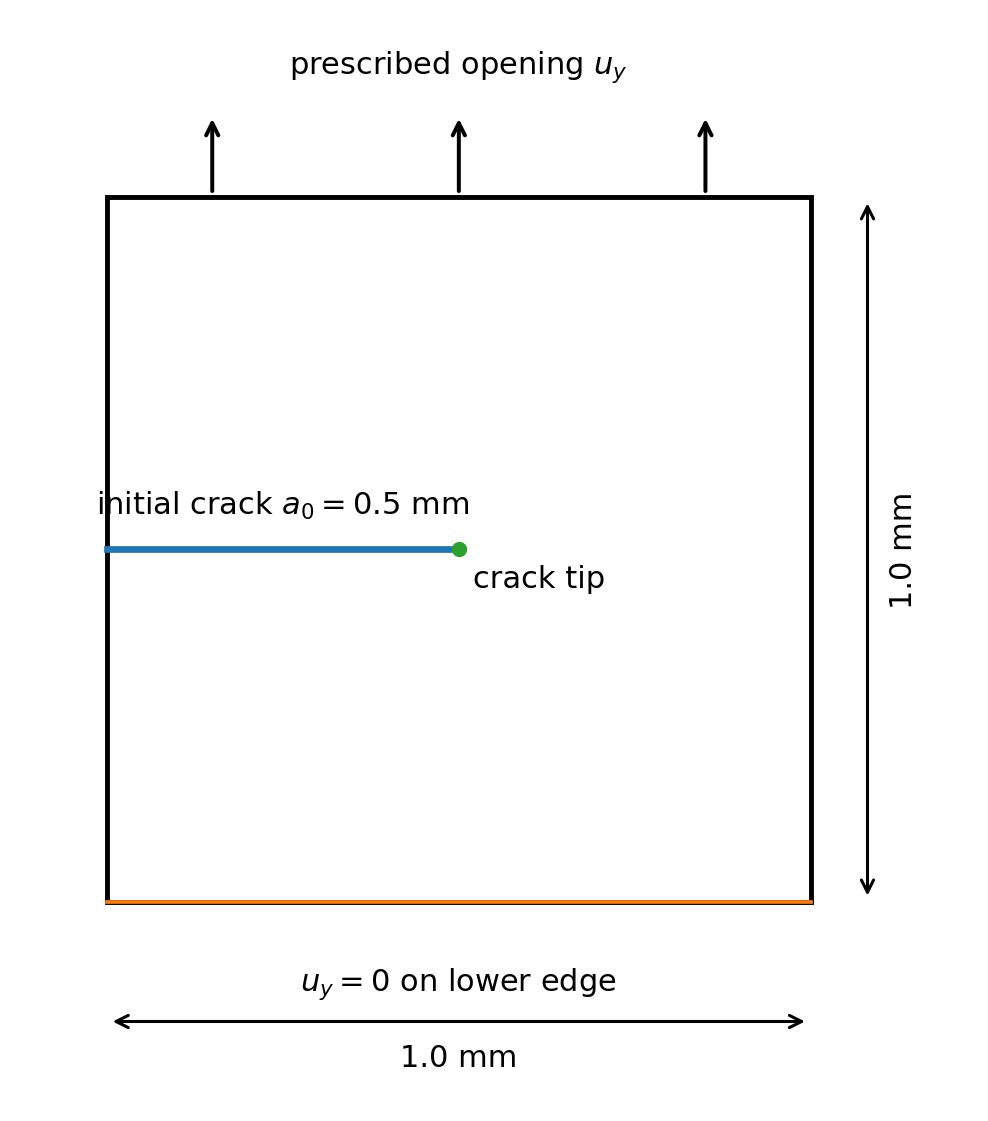
\includegraphics[width=0.36\textwidth]{fig_mode1_geometry.png}
  \caption{Mode-I fracture benchmark geometry: $1.0\times 1.0\,\mathrm{mm}$ plate with initial sharp slit seam ($a_0 = 0.5\,\mathrm{mm}$ along $y = 0.5\,\mathrm{mm}$, $0 \le x \le 0.5\,\mathrm{mm}$), roller bottom support with pinned origin, and prescribed top tensile displacement.}
  \label{fig:mode1_geometry}
\end{figure}

\subsubsection{Geometry and Sharp Seam Representation}
The computational domain is a unit square plate $\Omega = [0, 1] \times [0, 1]\,\mathrm{mm}$ containing an initial horizontal crack of length $a_0 = 0.5\,\mathrm{mm}$ along the symmetry line $y = 0.5\,\mathrm{mm}$ ($0 \le x \le 0.5\,\mathrm{mm}$). 
\begin{quote}
\textbf{Essential Benchmark Representation:} The crack is represented as a \textbf{zero-gap sharp seam} with coincident but geometrically distinct, uncoupled duplicate node pairs along the upper and lower crack flanks. Earlier exploratory models utilizing a finite-width notch radically increased compliance ($K_0 \approx 75.5\,\mathrm{kN/mm}$) and are strictly superseded; the zero-gap sharp seam is the mandatory benchmark representation.
\end{quote}

\subsubsection{Material and Phase-Field Regularization Parameters}
The constitutive response follows isotropic linear elasticity coupled to the AT2 phase-field damage formulation:
\begin{itemize}[leftmargin=4mm,itemsep=1pt,topsep=1pt]
  \item Young's modulus: $E = 210\,\mathrm{GPa} = 210\,\mathrm{kN/mm^2}$
  \item Poisson's ratio: $\nu = 0.3$
  \item Critical energy release rate (fracture toughness): $G_c = 2.7 \times 10^{-3}\,\mathrm{kN/mm} = 2.7\,\mathrm{N/mm}$
  \item Phase-field regularization length scale: $\ell_0 = 0.0075\,\mathrm{mm} = 7.5\,\mu\mathrm{m}$
\end{itemize}

\subsubsection{Boundary Conditions and Kinematics}
The specimen is loaded monotonically under displacement control:
\begin{itemize}[leftmargin=4mm,itemsep=1pt,topsep=1pt]
  \item \textbf{Bottom Boundary ($y = 0.0\,\mathrm{mm}$):} Roller support constraining vertical motion ($u_y = 0$). To prevent rigid body translation, the origin node at $(0, 0)$ is pinned ($u_x = 0, u_y = 0$).
  \item \textbf{Top Boundary ($y = 1.0\,\mathrm{mm}$):} Prescribed uniform vertical tensile displacement $u_y = u$, with lateral displacement constrained ($u_x = 0$, clamped tension).
\end{itemize}

\subsubsection{Expected Physical Response}
The anticipated physical response comprises four distinct regimes:
\begin{enumerate}[leftmargin=4mm,itemsep=1pt,topsep=1pt]
  \item \textbf{Linear Elastic Loading:} Initial linear elastic deformation with global structural stiffness $K_0 \approx 138\,\mathrm{kN/mm}$ governed by plate geometry and elastic constants.
  \item \textbf{Sub-Critical Damage Localization:} Growth of the continuous damage parameter $d \in [0, 1]$ within an inner process zone of width $\sim 2\ell_0$ directly ahead of the crack tip $(0.5, 0.5)\,\mathrm{mm}$.
  \item \textbf{Peak Load and Instability:} Attainment of peak reaction force $F_{\max} \approx 0.758\,\mathrm{kN}$ at $u(F_{\max}) \approx 0.00586\,\mathrm{mm}$.
  \item \textbf{Post-Peak Softening and Propagation:} Rapid load drop as the crack extends horizontally along the line of symmetry $y = 0.5\,\mathrm{mm}$ towards the right boundary ($x = 1.0\,\mathrm{mm}$).
\end{enumerate}

\subsection{Fixed-Mesh Reference Solution as Quantitative Anchor}
To establish an authoritative baseline against which all adaptive remeshing results are judged, a conventional fixed-mesh simulation was executed (Job \texttt{1398090.mmaster02}). 

\begin{quote}
\textbf{Mandatory Anchor Statement:} \emph{``This fixed-mesh solution is the reference response that any adaptive solution must reproduce to an acceptable accuracy.''} Everything after that must be measured against it.
\end{quote}

The reference mesh comprises $15{,}192$ linear quadrilateral finite elements (\texttt{CPE4}), with a uniformly refined crack corridor satisfying $h \approx 0.0015\,\mathrm{mm} \le \ell_0 / 5$, guaranteeing resolution of diffuse phase gradients. 

\begin{table}[htbp]
  \centering
  \footnotesize
  \caption{Quantitative comparison between published literature and reconstructed fixed reference anchor.}
  \label{tab:reference_anchor}
  \begin{tabularx}{\textwidth}{L{46mm} C{28mm} C{28mm} C{24mm}}
    \toprule
    \textbf{Quantity} & \textbf{Literature Target} \citep{Pandey2025} & \textbf{Reconstructed Ref.} (\texttt{1398090}) & \textbf{Relative Error} \\
    \midrule
    Number of finite elements & $\sim 15{,}000$ & $15{,}192$ & $+1.28\%$ \\
    Peak reaction force $F_{\max}$ & $0.7580\,\mathrm{kN}$ & $0.757778\,\mathrm{kN}$ & $-0.029\%$ \\
    Displacement at peak $u(F_{\max})$ & $0.005860\,\mathrm{mm}$ & $0.005857\,\mathrm{mm}$ & $-0.051\%$ \\
    Initial stiffness $K_0$ (OLS, $u \le 1.0\,\mu\mathrm{m}$) & -- & $137.945520\,\mathrm{kN/mm}$ & Baseline Anchor \\
    OLS coefficient of determination $R^2$ & -- & $0.99999960$ ($N=400$) & Baseline Anchor \\
    OLS intercept $F_0$ & -- & $4.472368 \times 10^{-5}\,\mathrm{kN}$ & Baseline Anchor \\
    Final load drop at $u = 0.010\,\mathrm{mm}$ & $>98\%$ & $99.97\%$ ($0.23\,\mathrm{N}$) & Severed \\
    \bottomrule
  \end{tabularx}
\end{table}

\subsubsection{Rigorous Definition of Initial Structural Stiffness \texorpdfstring{$K_0$}{K0}}
In this report, the initial stiffness $K_0$ is defined as the unconstrained Ordinary Least Squares (OLS) slope with intercept fitted over the initial elastic range $u \in [0, 0.0010]\,\mathrm{mm}$ ($400$ uniform increments):
\begin{equation}
\label{eq:ols_stiffness}
K_0 = \left.\frac{\mathrm{d}F}{\mathrm{d}u}\right|_{\mathrm{elastic}} = \frac{\sum_{i=1}^N (u_i - \bar{u})(F_i - \bar{F})}{\sum_{i=1}^N (u_i - \bar{u})^2} = 137.945520\,\mathrm{kN/mm} \quad (R^2 = 0.99999960).
\end{equation}
\begin{quote}
\textbf{Clarification on Historical Values:} Preliminary reports occasionally cited $K_0 \approx 138.084\,\mathrm{kN/mm}$ based on a 2-point secant slope between $u=0$ and $u=0.001\,\mathrm{mm}$. To prevent ambiguity, the authoritative unconstrained OLS value $K_0 = 137.945520\,\mathrm{kN/mm}$ is adopted strictly across all subsequent comparisons. $K_0$ represents a global structural stiffness, distinct from the intrinsic material Young's modulus $E = 210\,\mathrm{GPa}$.
\end{quote}

\subsubsection{Multifaceted Mesh-Convergence Assessment}
Peak reaction force ($F_{\max}$) alone is strictly insufficient to demonstrate finite element convergence or model adequacy. Complete convergence evaluation requires:
\begin{enumerate}[leftmargin=4mm,itemsep=1pt,topsep=1pt]
  \item Complete force-displacement ($F$--$u$) curve tracking across the full range (elastic, peak, and softening);
  \item Initial structural stiffness $K_0$ and linearity ($R^2$);
  \item Peak reaction force $F_{\max}$ and displacement at peak $u(F_{\max})$;
  \item Spatial damage field $d(x, y)$ contours and process-zone localization profiles;
  \item Crack-path and localization-profile convergence along the ligament;
  \item Total external work $W_{\mathrm{ext}} = \int F\,\mathrm{d}u$.
\end{enumerate}

\begin{quote}
\textbf{Critical UEL Internal-Energy Balance Limitation:} As documented in Section~4.6 of the project audit, Abaqus' built-in \texttt{ENERGY} history array is not populated for user-defined finite elements (\texttt{UEL}). Consequently, an internal strain-energy vs fracture-energy balance cannot be extracted from standard solver outputs; the integrated measure $W_{\mathrm{ext}} = \int F\,\mathrm{d}u$ represents external mechanical work, not internal energy.
\end{quote}

\clearpage

\section{Pandey--Kumar Native Adaptive Remeshing Methodology}
\label{sec:adaptive_method_miseseri}

\subsection{Two-Job Pre-Refinement Workflow Architecture}
Pandey \& Kumar \citep{Pandey2025} proposed an adaptive mesh refinement scheme leveraging the built-in adaptive remeshing capabilities of Abaqus/Standard. The workflow operates as an automated two-stage procedure executed via Python scripting:
\begin{equation*}
\boxed{\text{Coarse Mesh}} \xrightarrow{\text{Job 1}} \boxed{\text{Elastic Pre-Analysis}} \xrightarrow{\text{Extract}} \boxed{\texttt{MISESERI}\text{ Field}} \xrightarrow{\text{Apply}} \boxed{\texttt{RemeshingRule}} \xrightarrow{\texttt{adaptiveRemesh()}} \boxed{\text{Adapted Mesh}} \xrightarrow{\text{Job 2}} \boxed{\text{Fracture Solve}}
\end{equation*}

\begin{enumerate}[label=\textbf{Step \arabic*:},leftmargin=18mm,itemsep=1pt,topsep=1pt]
  \item \textbf{Coarse Mesh Generation:} The domain $\Omega$ is discretized with a coarse global seed $h_{\mathrm{cms}} = 0.020\,\mathrm{mm}$, containing the initial sharp crack seam.
  \item \textbf{Linear Elastic Pre-Analysis (Job 1):} A standard elastic solve is executed under prescribed Mode-I tensile stroke. Because no user elements or damage evolutions are active, this step solves in seconds.
  \item \textbf{Error Indicator Evaluation:} Abaqus calculates the recovered stress discretization error indicator \texttt{MISESERI} across the domain.
  \item \textbf{Abaqus Remeshing Rule Execution:} An Abaqus Python script defines a \texttt{RemeshingRule} and invokes \texttt{adaptiveRemesh()}, generating a new mesh tailored to reduce stress discretization error.
  \item \textbf{UEL/UMAT Layer Reconstruction:} Python scripts parse the adapted mesh and generate coincident co-located \texttt{UEL} user elements and companion visualization \texttt{UMAT} elements.
  \item \textbf{Phase-Field Fracture Simulation (Job 2):} The final nonlinear fracture simulation is executed on the refined mesh using the user-defined element formulation.
\end{enumerate}

\subsection{Canonical Mode-I Pre-Analysis Mesh \& Error Extraction}
A rigorous audit of the source pre-analysis deck established the canonical baseline:
\begin{itemize}[leftmargin=4mm,itemsep=1pt,topsep=1pt]
  \item \textbf{Mesh Discretization:} Exactly $2{,}906$ finite elements ($2{,}818$ quadrilateral \texttt{CPE4} elements and $88$ triangular \texttt{CPE3} transition elements), defined by $2{,}988$ nodes.
  \item \textbf{Seam Topology:} Zero-gap sharp slit seam ($a_0 = 0.5\,\mathrm{mm}$) with duplicate coincident nodes on upper and lower flanks.
  \item \textbf{Extracted Error Records:} Direct inspection of \texttt{JOB1\_LOAD\_1p0X.odb} confirmed that the field output contains exactly \textbf{$2{,}906$ scalar values} at the \texttt{WHOLE\_ELEMENT} position ($1$ value per finite element).
\end{itemize}

\begin{quote}
\textbf{Resolution of Obsolete Provenance Data:} In the preliminary 02 September report, Figure~3.1 erroneously plotted a $3{,}930$-row dataset extracted from Job \texttt{1379893.mmaster02}. That run belonged to the earlier Mode-II shear mesh, not the canonical Mode-I pre-analysis. That obsolete dataset is formally retired and replaced with the verified $2{,}906$-element Mode-I field shown in Figure~\ref{fig:miseseri_canonical}.
\end{quote}

\begin{figure}[htbp]
  \centering
  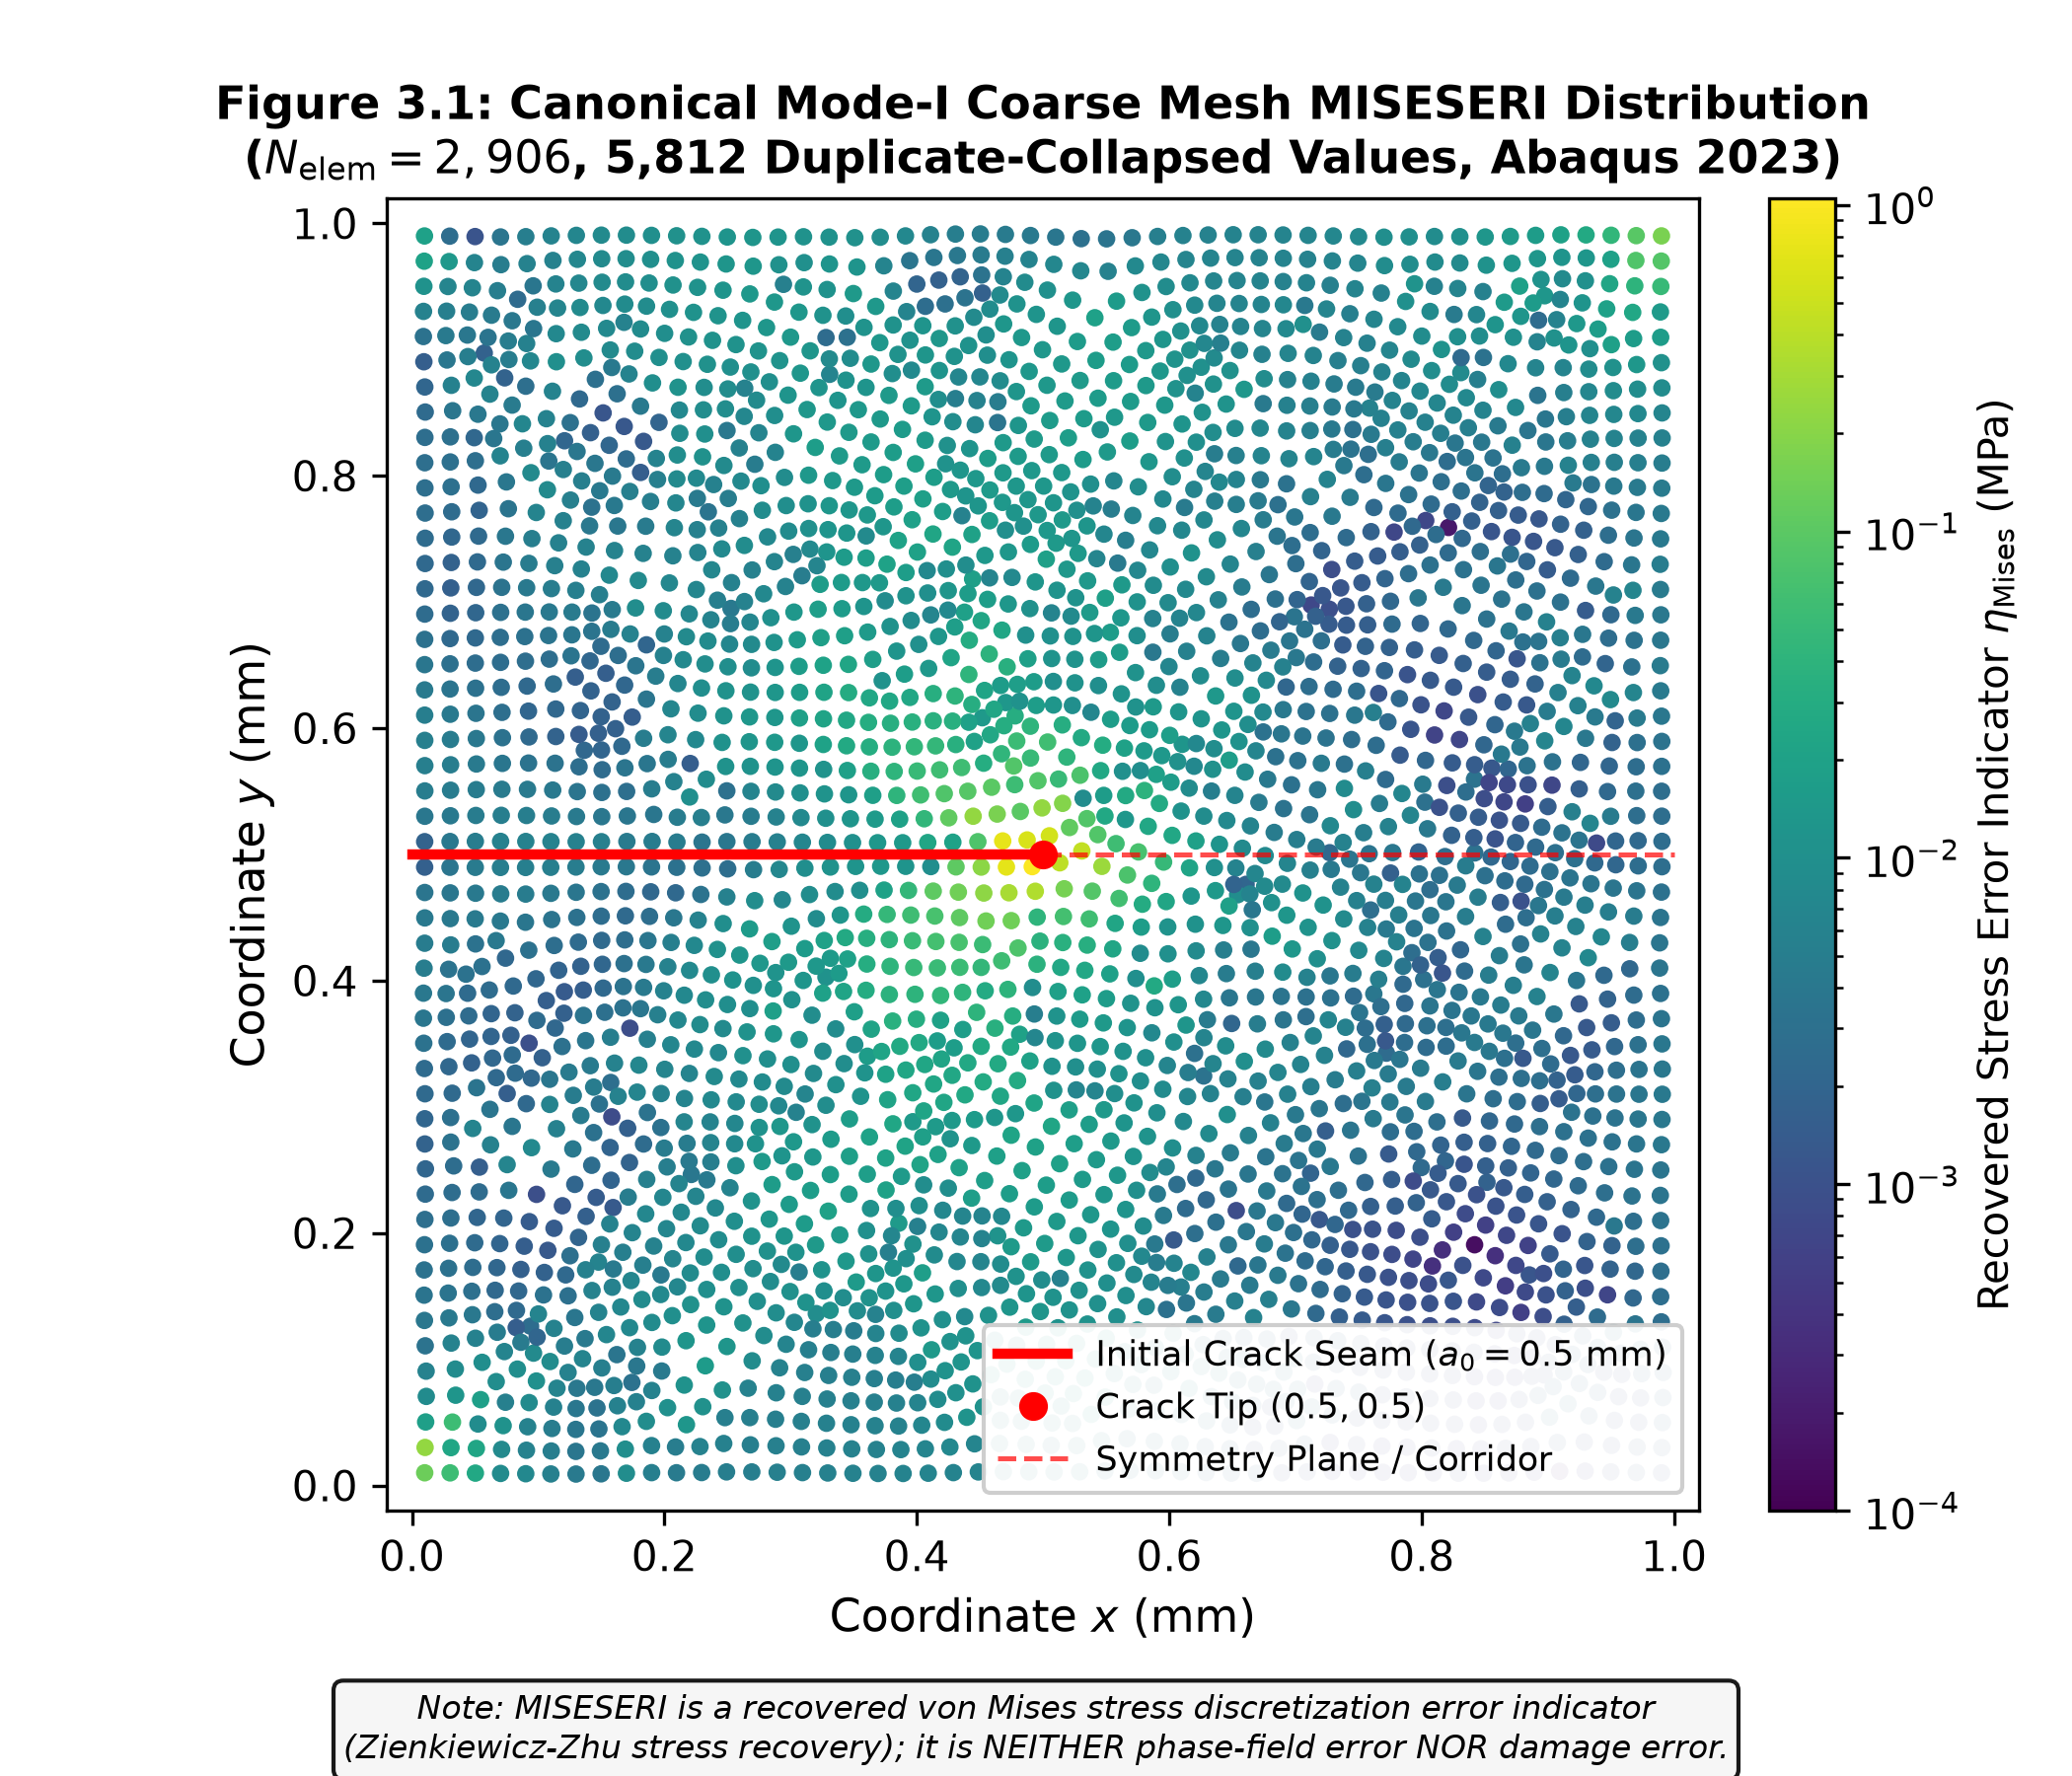
\includegraphics[width=0.68\textwidth]{figure_3_1_canonical_mode1_miseseri_error_map.png}
  \caption{Canonical Mode-I pre-analysis von Mises stress discretization error indicator (\texttt{MISESERI}) field ($2{,}906$ finite elements). Error is sharply peaked at the singular crack tip ($\max = 1.007\,\mathrm{MPa}$), while remaining low in far-field regions ($\mathrm{median} = 5.78 \times 10^{-3}\,\mathrm{MPa}$).}
  \label{fig:miseseri_canonical}
\end{figure}

\subsection{Physical Meaning and Epistemic Limits of MISESERI}
It is essential to maintain absolute scientific clarity regarding what \texttt{MISESERI} represents:
\begin{itemize}[leftmargin=4mm,itemsep=1pt,topsep=1pt]
  \item \textbf{Definition:} \texttt{MISESERI} is the Abaqus stress discretization/error indicator associated with the recovered von Mises stress field \citep{Abaqus2023}; it is not a phase-field or damage error indicator.
  \item \textbf{Epistemic Scope:} It measures stress discretization error in the linear-elastic pre-analysis rather than damage evolution or crack propagation.
  \item \textbf{Abaqus Internal Sizing Transformation:} While \texttt{MISESERI} guides mesh sizing, the exact transformation algorithms, smoothing filters, and element-growth constraints internal to \texttt{adaptiveRemesh} remain undocumented proprietary routines of the Abaqus kernel \citep{Abaqus2023}. We report verified numerical outputs rather than conjecturing undocumented internal formulas.
\end{itemize}

\subsection{Published Remeshing Rule Implementation}
To guarantee literal adherence to the published method, the Abaqus remeshing rule is scripted exactly as specified in Listing~1 of Pandey \& Kumar \citep{Pandey2025}:
\begin{itemize}[leftmargin=4mm,itemsep=1pt,topsep=1pt]
  \item Error indicator variable: \texttt{variables=('MISESERI',)}
  \item Sizing method: \texttt{sizingMethod=UNIFORM\_ERROR}
  \item Error target: \texttt{errorTarget=1.0} (representing $1.0\%$ relative stress error)
  \item Element size bounds: \texttt{minElementSize=0.001}, \texttt{maxElementSize=0.020}
  \item Refinement dynamics: \texttt{refinementFactor=10}, \texttt{coarseningFactor=NOT\_ALLOWED}
  \item Output frequency: \texttt{outputFrequency=ALL\_INCREMENTS}
  \item Remeshing domain: Whole specimen (\texttt{All\_elem})
\end{itemize}
Applying this literal rule to the canonical Mode-I pre-analysis produces an adapted mesh of $71{,}320$ finite elements.

\clearpage

\section{Resolution of the 71,320-Element Stiffness Anomaly (Priority Question A)}
\label{sec:stiffness_anomaly_resolution}

\subsection{Historical Anomaly and Initial Hypotheses}
In earlier project reports, the nominal 1\% 71,320-element adaptive fracture simulation (Job \texttt{1399632.mmaster02}) completed technically but exhibited an alarming mechanical discrepancy:
\begin{itemize}[leftmargin=4mm,itemsep=1pt,topsep=1pt]
  \item Initial structural stiffness dropped from the reference $K_0 = 137.95\,\mathrm{kN/mm}$ down to $K_0 \approx 122.38\,\mathrm{kN/mm}$ ($-11.3\%$).
  \item Peak reaction force collapsed from $0.758\,\mathrm{kN}$ to $F_{\max} = 0.478203\,\mathrm{kN}$ ($-36.9\%$).
\end{itemize}
Because this run employed companion visualization elements and non-symmetric Newton solver settings (\texttt{UNSYMM=YES}), preliminary analyses speculated that co-located element coupling, Fortran common block collisions, or formulation asymmetry caused the stiffness deficit. Controlled one-factor diagnostics were mandated to isolate the exact equation-level cause.

\subsection{Forensic Equation-Level Audit: The 16-Entry Parser Limit}
A comprehensive boundary set audit of the runtime output databases (Job \texttt{1404312.mmaster02}) revealed the true mathematical defect, entirely unrelated to UEL formulations or adaptive remeshing:
\begin{enumerate}[leftmargin=4mm,itemsep=1pt,topsep=1pt]
  \item \textbf{Abaqus Input Preprocessor Truncation Limit:} Under free-format \texttt{*NSET} cards without the \texttt{GENERATE} parameter, the Abaqus input preprocessor (\texttt{pre}) strictly enforces a maximum of \textbf{16 node entries per line} \citep{Abaqus2023}.
  \item \textbf{Card Formatting Defect:} In the Python mesh generation script, the bottom roller node set \texttt{N\_BOTTOM} was written as a single line containing all $150$ node identifiers.
  \item \textbf{Parser Preprocessing Warnings and Set Truncation:} Abaqus issued preprocessing warnings and retained only 16 of the intended 150 \texttt{N\_BOTTOM} node IDs; the remaining 134 entries were deleted from the parsed set.
  \item \textbf{Unconstrained Kinematic Boundary:} The vertical roller constraint ($u_y = 0$) was omitted for all 134 deleted nodes. Over $89\%$ of the bottom boundary was left completely unconstrained in the vertical direction.
\end{enumerate}

\begin{figure}[htbp]
  \centering
  \begin{minipage}{0.48\textwidth}
    \centering
    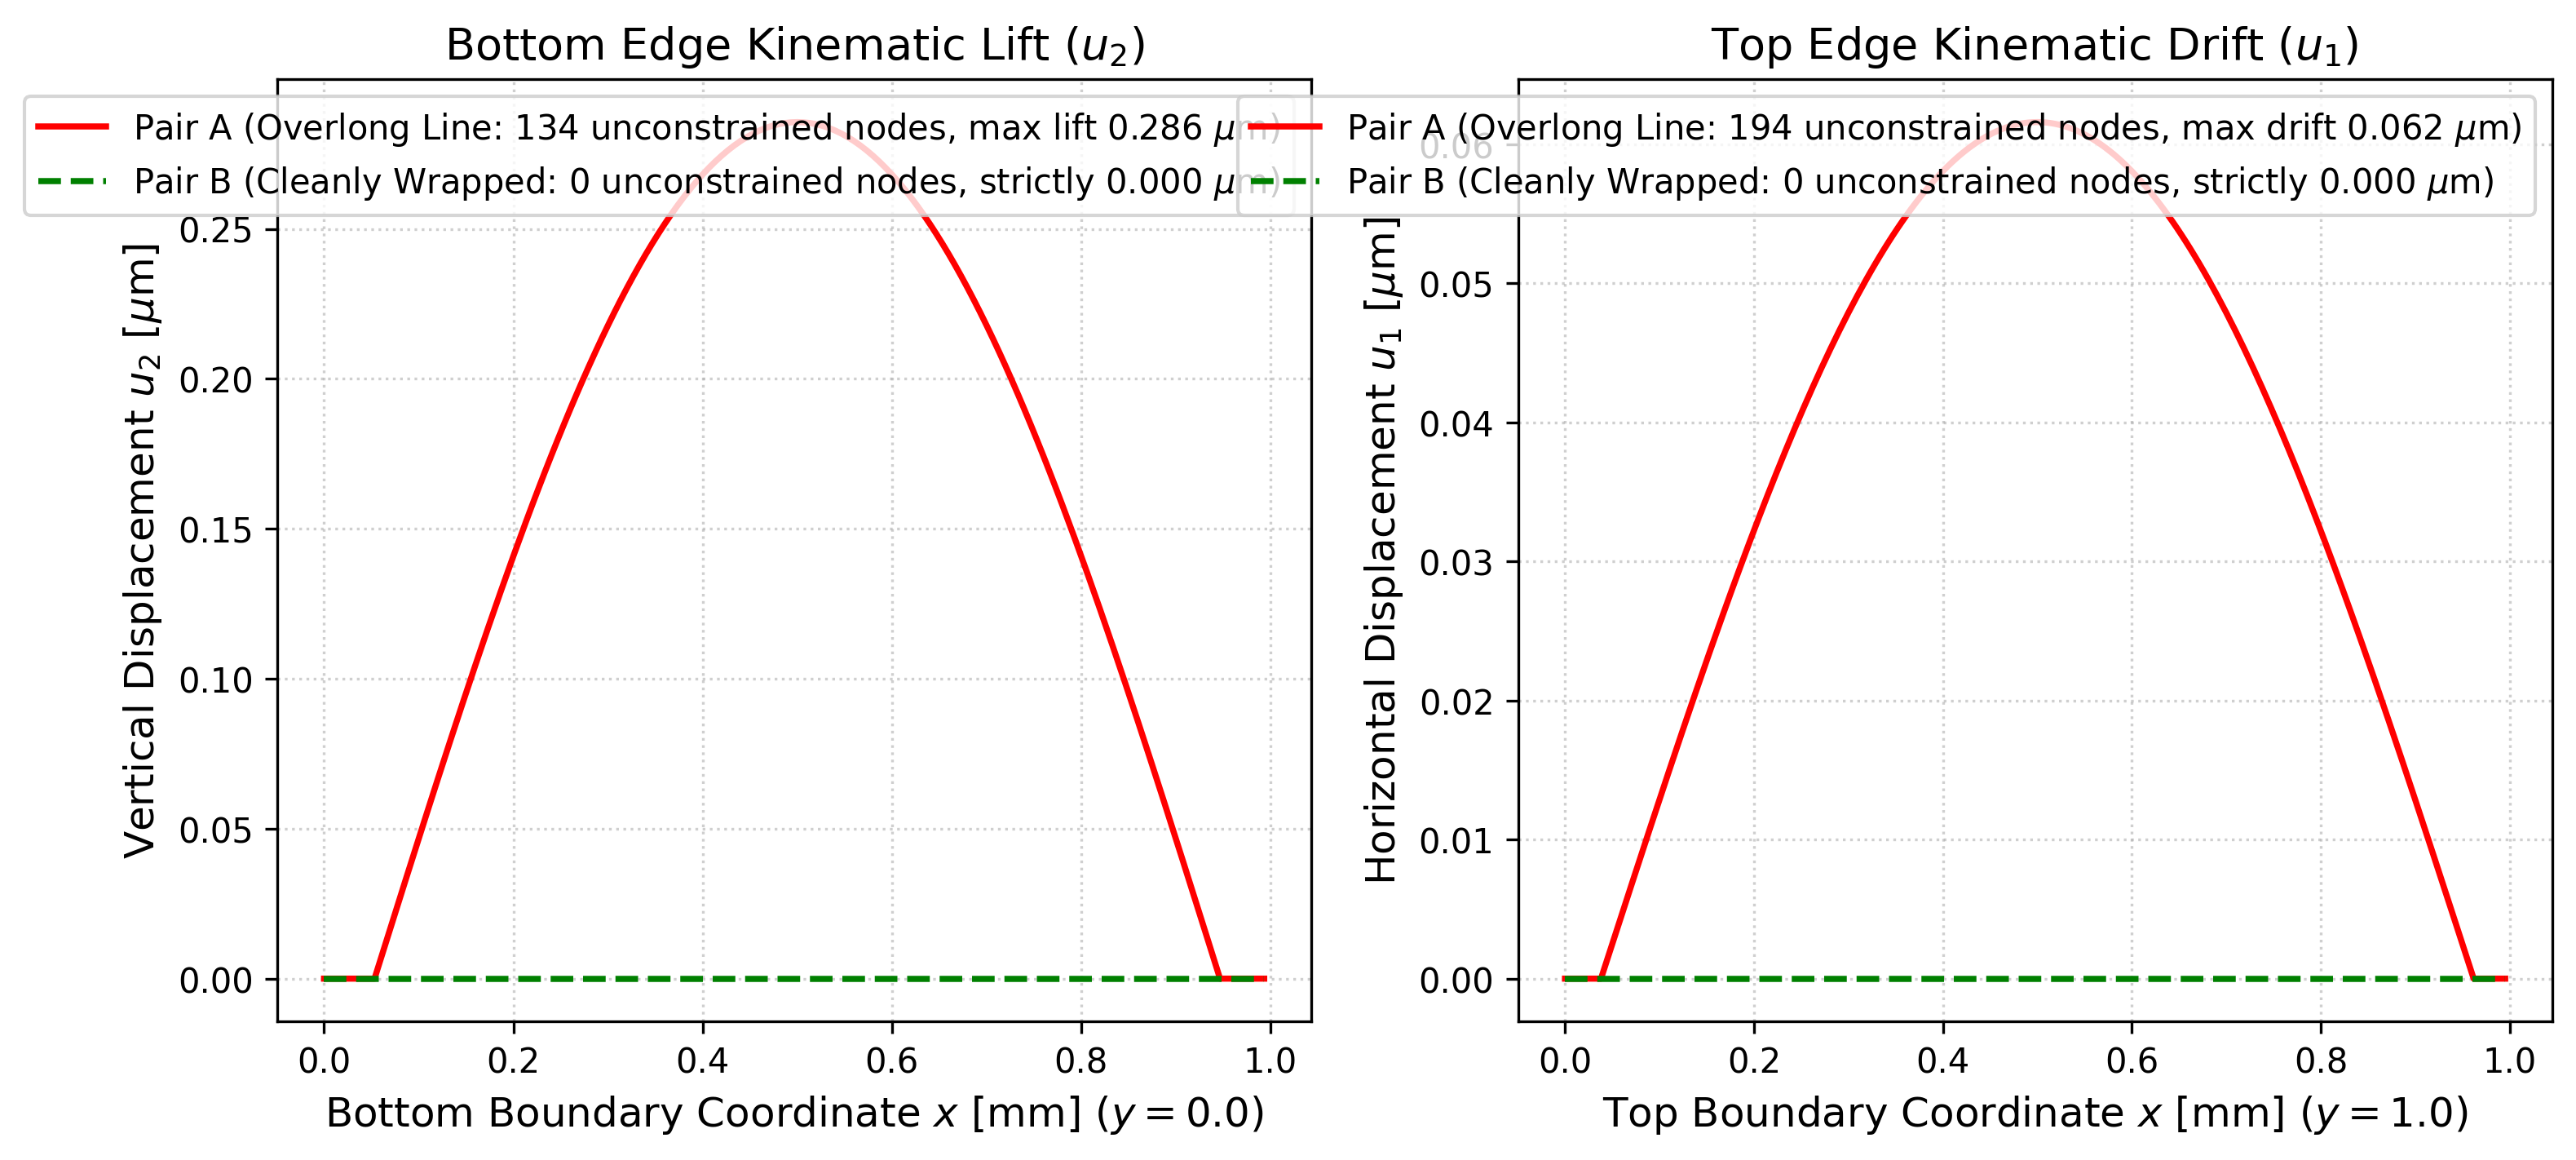
\includegraphics[width=\textwidth]{fig3_boundary_truncation_mechanism.png}
    \caption*{(a) 16-node card truncation mechanism.}
  \end{minipage}\hfill
  \begin{minipage}{0.48\textwidth}
    \centering
    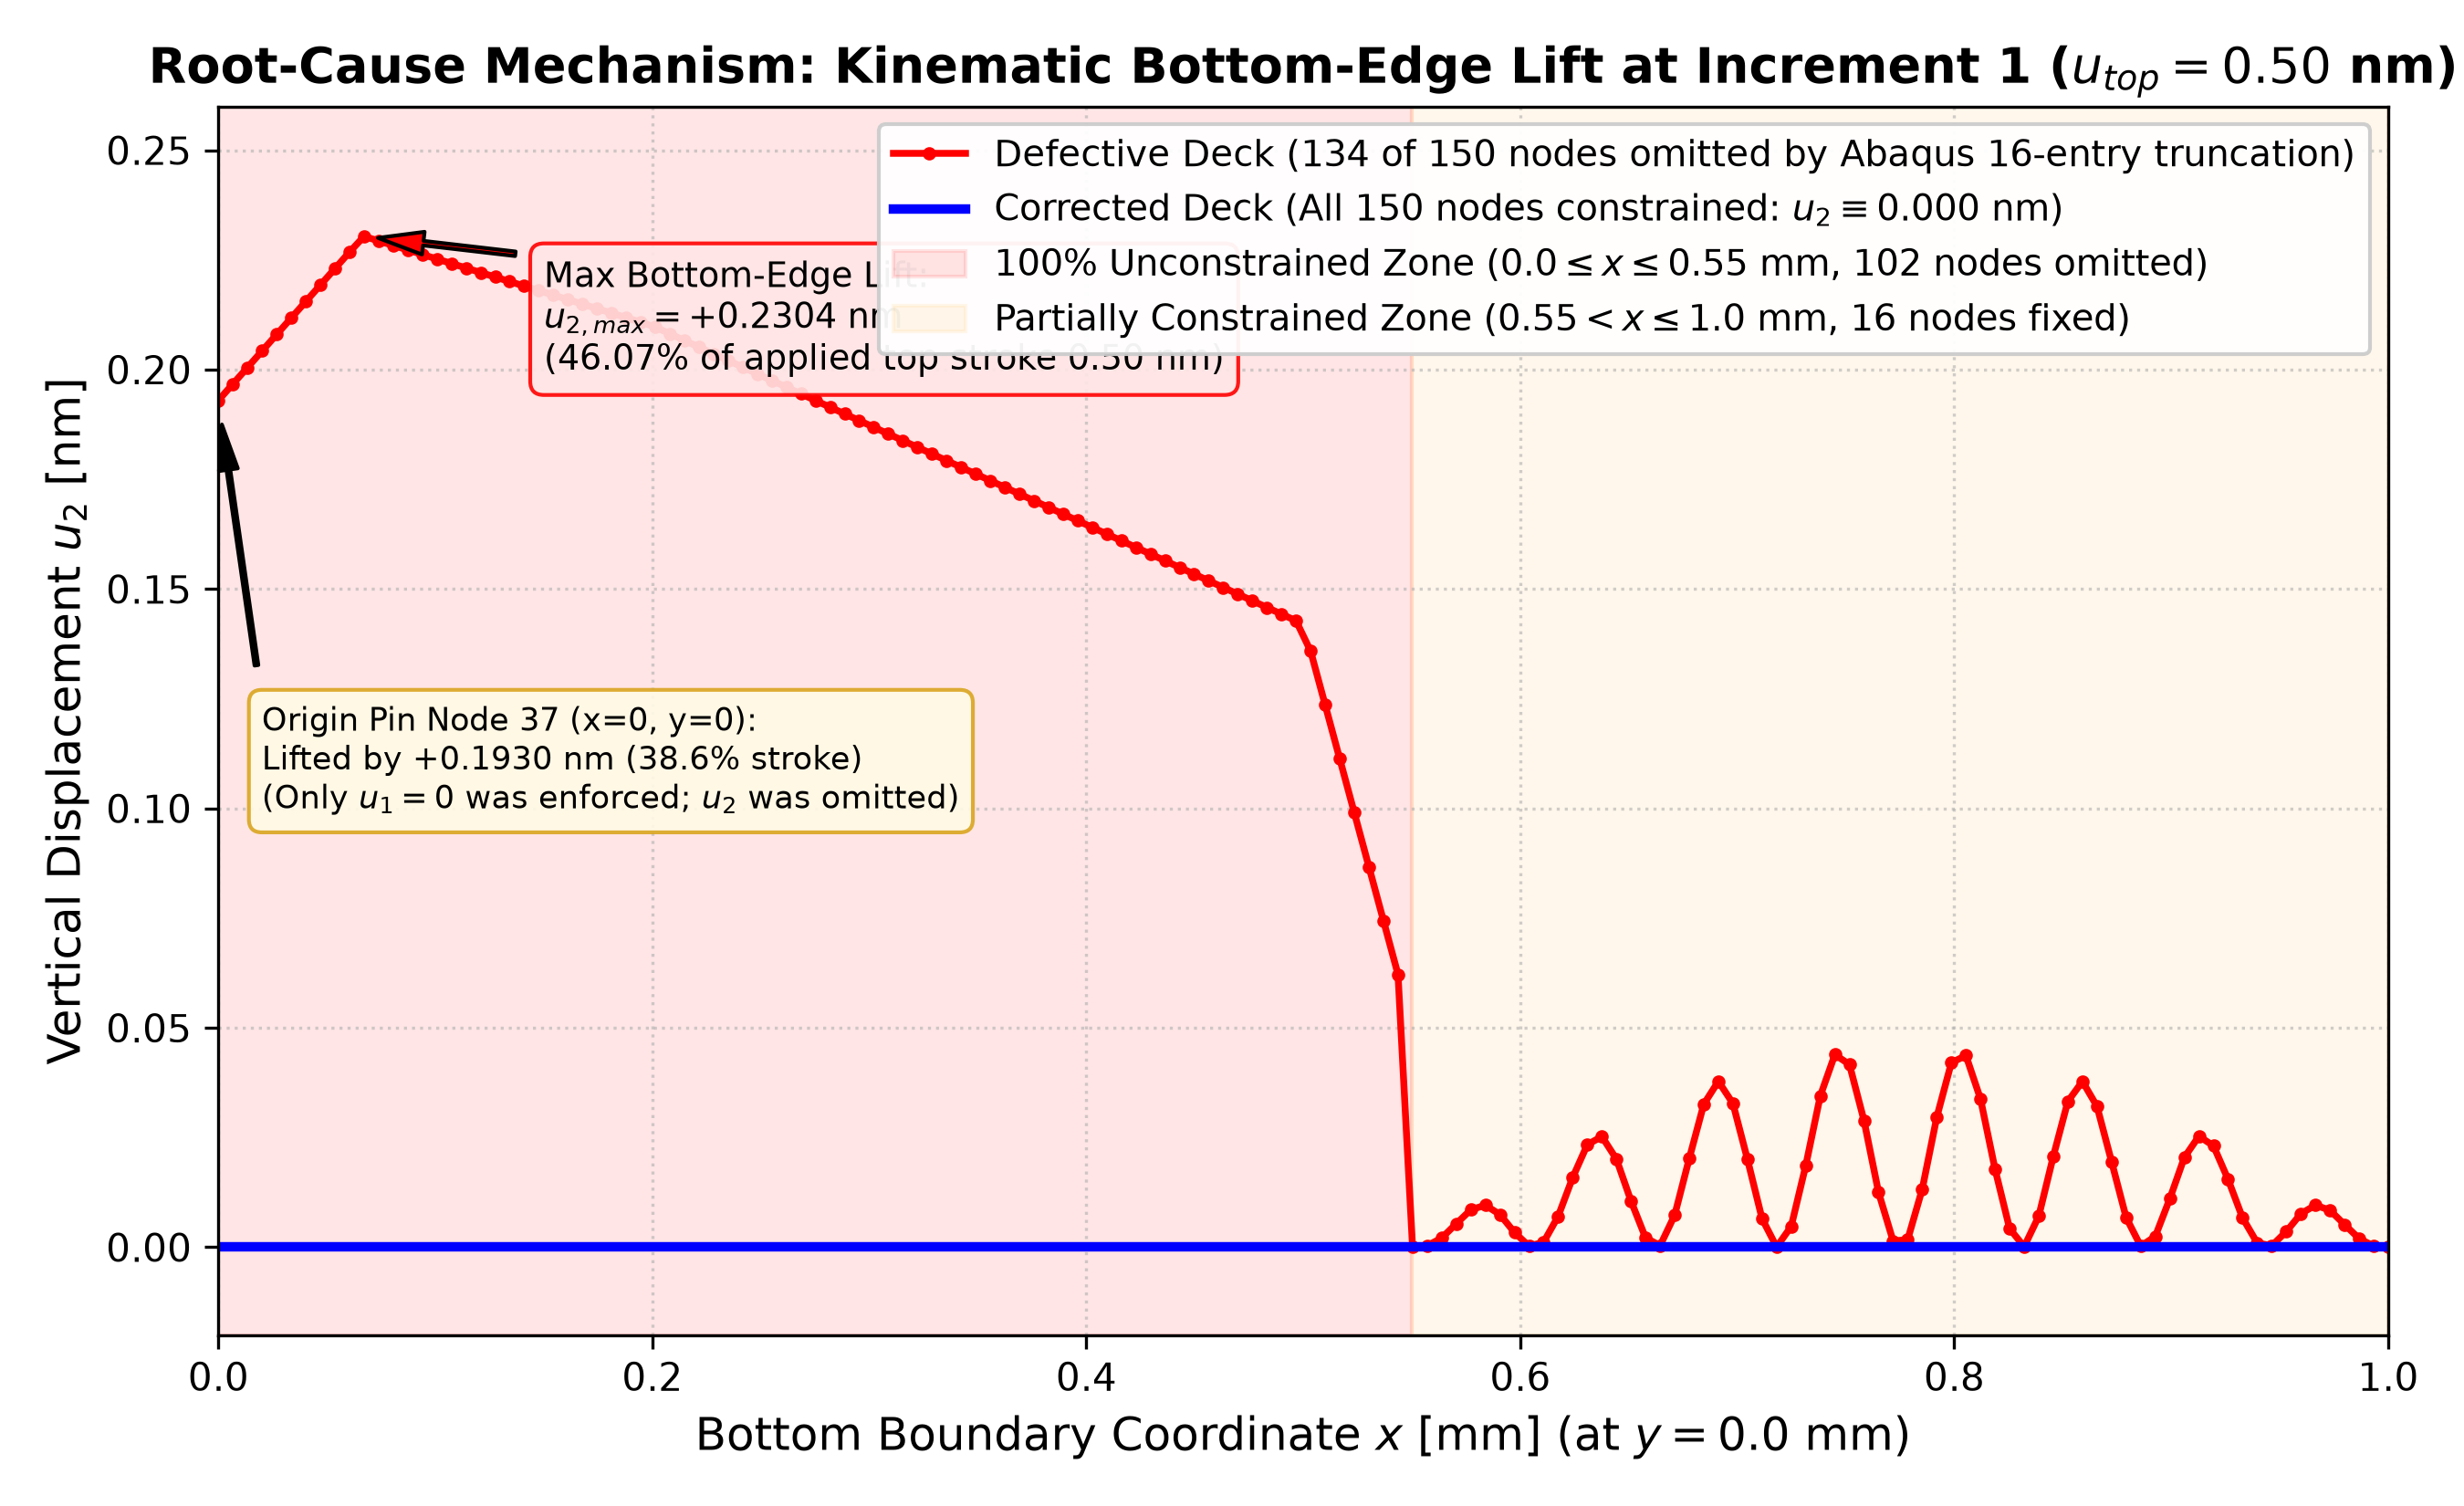
\includegraphics[width=\textwidth]{fig3_bottom_edge_lift_kinematics.png}
    \caption*{(b) Resulting bottom-edge lift profile $u_2(x)$.}
  \end{minipage}
  \caption{Kinematic mechanism of the stiffness anomaly: 134 unconstrained bottom nodes allowed bottom-edge vertical lift up to approximately $48.34\%$ of the applied stroke, inducing artificial structural compliance.}
  \label{fig:truncation_mechanism}
\end{figure}

\subsubsection{Kinematic Mechanism: Bottom-Edge Lift}
Extraction of nodal displacements demonstrated that the malformed case permitted bottom-edge vertical lift up to approximately $48.34\%$ of the applied stroke, whereas the corrected case constrained all 150 intended bottom nodes to $u_2=0$ (Figure~\ref{fig:truncation_mechanism}). This unconstrained boundary compliance artificially reduced reaction forces, producing the apparent low-stiffness branch ($122.38\,\mathrm{kN/mm}$).

\begin{quote}
\textbf{Controlled Parser Verification (Job \texttt{1404318}):} A minimal controlled test verified that this 16-item limit is a general feature of the Abaqus input syntax. Furthermore, the hypothesis \texttt{FACTORIAL\_UNSYMM\_X\_COMPANION} is formally \textbf{\texttt{RETRACTED}}; companion elements cause $0.000\%$ stiffness change.
\end{quote}

\subsection{Recovery, Requalification, and Production Validation}
Formatting all \texttt{*NSET} records with $\le 16$ items per line completely restored all 150 boundary constraints, eliminating bottom-edge lift ($u_2 \equiv 0.000\,\mathrm{nm}$) and recovering stiffness immediately:
\begin{itemize}[leftmargin=4mm,itemsep=1pt,topsep=1pt]
  \item \textbf{Corrected Frozen 71,320 Requalification (Job \texttt{1405044}):} Initial stiffness restored to $K_0 = \mathbf{138.021013\,\mathrm{kN/mm}}$ ($+0.0547\%$ vs reference anchor $137.945520\,\mathrm{kN/mm}$), with all 150/150 bottom nodes constrained and zero set-truncation or deletion warnings in solver diagnostics.
  \item \textbf{Corrected Full-Fracture Nominal 1\% (Job \texttt{1404933}):} Reached $F_{\max} = \mathbf{0.745325\,\mathrm{kN}}$ at $u(F_{\max}) = \mathbf{0.005750\,\mathrm{mm}}$, with initial stiffness $K_0 \approx \mathbf{137.821\,\mathrm{kN/mm}}$ ($137.820804\,\mathrm{kN/mm}$, $-0.0904\%$ vs reference anchor).
  \item \textbf{Stage-A Shared-Memory Thread Parity (Job \texttt{1405003}):} 4-thread execution reproduced serial results within tight numerical parity (Stage-B repeat pending).
\end{itemize}

\begin{figure}[htbp]
  \centering
  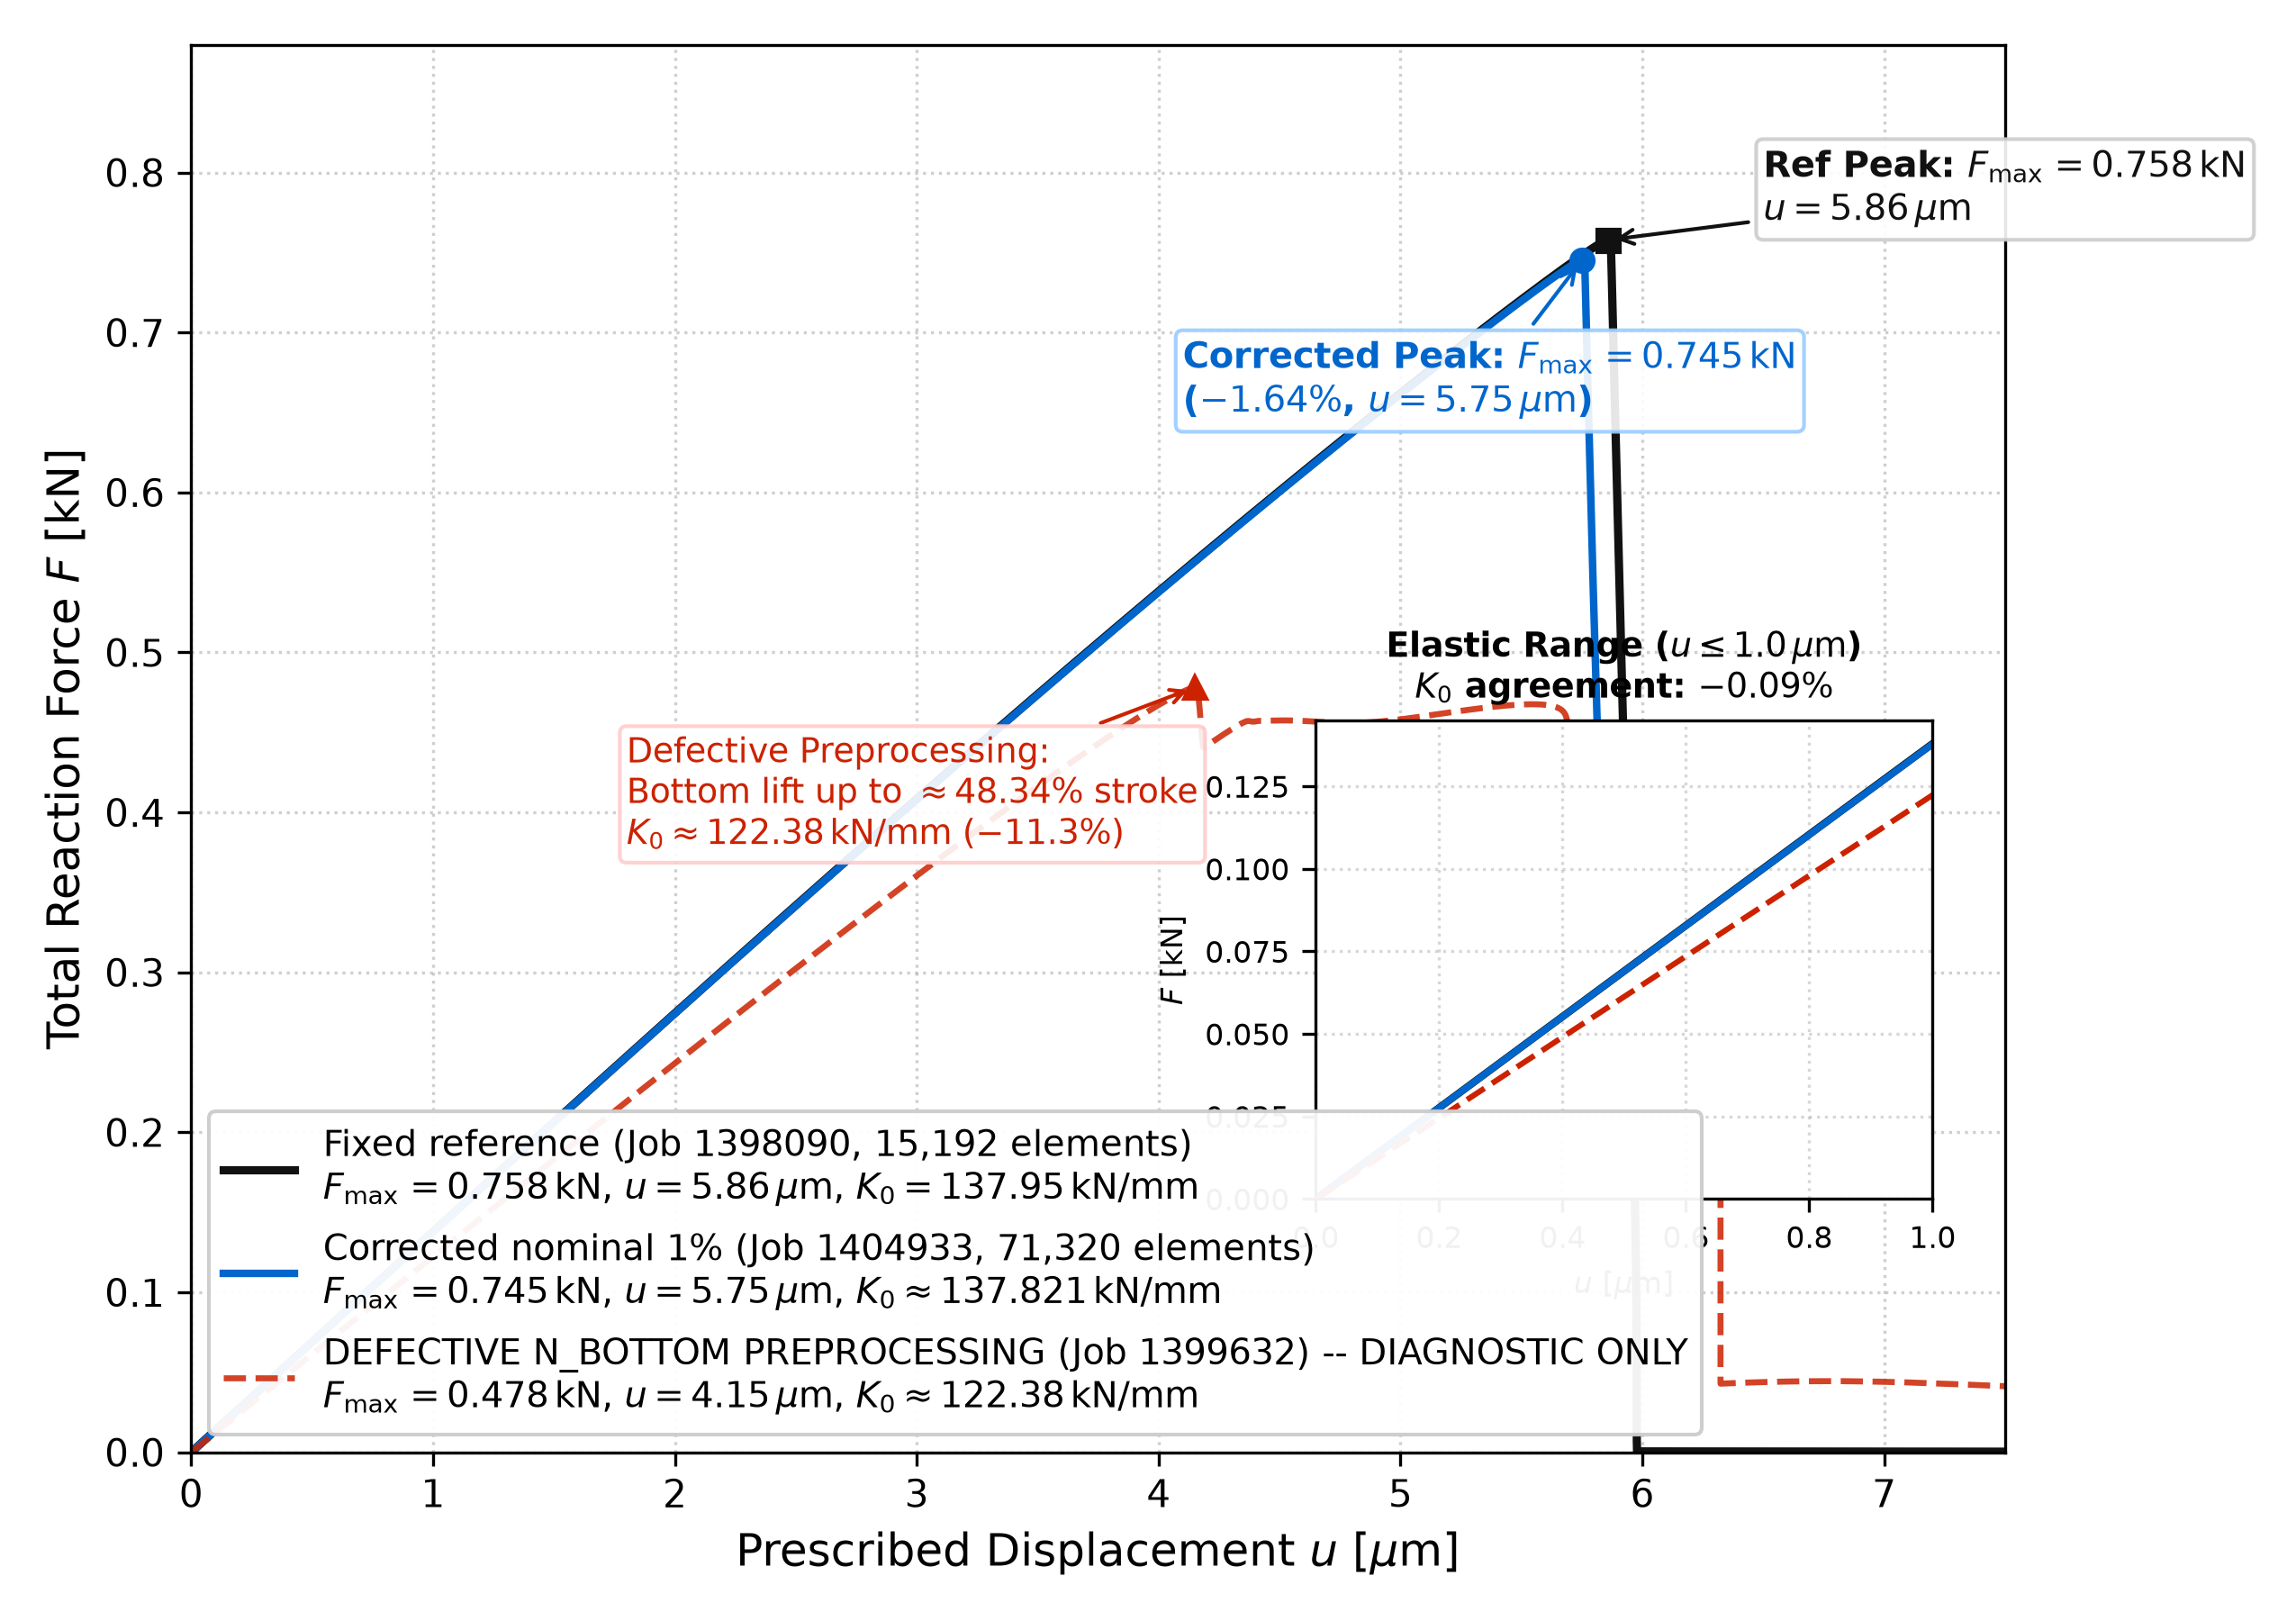
\includegraphics[width=0.70\textwidth]{fig1_mode1_fu_recovery.png}
  \caption{Mandatory Figure 1: Global force-displacement ($F$--$u$) response comparing the fixed reference anchor (Job \texttt{1398090}, $15{,}192$ elements) against the corrected nominal 1\% adaptive model (Job \texttt{1404933}, $71{,}320$ elements) and the historical predecessor (Job \texttt{1399632}, DEFECTIVE N\_BOTTOM PREPROCESSING -- DIAGNOSTIC ONLY). Inset confirms exact initial stiffness recovery ($K_0 \approx 137.821\,\mathrm{kN/mm}$, $-0.09\%$ vs reference $137.946\,\mathrm{kN/mm}$).}
  \label{fig:fu_overlay}
\end{figure}

\begin{table}[htbp]
  \centering
  \footnotesize
  \caption{Authoritative comparison of Mode-I mechanical response across key simulation jobs.}
  \label{tab:mode1_stiffness_summary}
  \begin{tabularx}{\textwidth}{L{48mm} C{18mm} C{22mm} C{22mm} C{22mm}}
    \toprule
    \textbf{Simulation Model} & \textbf{Elements} & $K_0$ \textbf{[kN/mm]} & $F_{\max}$ \textbf{[kN]} & $u(F_{\max})$ \textbf{[mm]} \\
    \midrule
    \textbf{Fixed Reference Anchor} (\texttt{1398090}) & $15{,}192$ & $137.946$ & $0.757778$ & $0.005857$ \\
    \textbf{DEFECTIVE N\_BOTTOM PREPROC.} (\texttt{1399632})\newline\textit{(DIAGNOSTIC ONLY)} & $71{,}320$ & $122.379$ ($-11.28\%$) & $0.478203$ ($-36.89\%$) & $0.004150$ \\
    \textbf{Corrected Frozen 71k} (\texttt{1405044}) & $71{,}320$ & $138.021$ ($+0.05\%$) & -- (elastic) & -- (elastic) \\
    \textbf{Corrected Nominal 1\%} (\texttt{1404933}) & $71{,}320$ & $137.821$ ($-0.09\%$) & $0.745325$ ($-1.64\%$) & $0.005750$ \\
    \textbf{Supporting 4T Twin} (\texttt{1405003}) & $71{,}320$ & $137.821$ ($-0.09\%$) & $0.745325$ ($-1.64\%$) & $0.005750$ \\
    \bottomrule
  \end{tabularx}
\end{table}

\begin{quote}
\textbf{Conclusion on Priority Question A:} Priority Question A is \textbf{\texttt{RESOLVED\_AND\_CLOSED}}. The 71,320-element adaptive mesh reproduces the fixed reference structural stiffness within $0.09\%$. The mechanical discrepancy is definitively closed.
\end{quote}

\clearpage

\section{The Reproduction Discrepancy: 71,320 vs \texorpdfstring{$\approx 13{,}941$}{approx. 13,941} (Priority Question B)}
\label{sec:discrepancy_audit_71k_vs_14k}

\subsection{Statement of the Reproduction Discrepancy}
The central remaining scientific question in reproducing the Pandey \& Kumar \citep{Pandey2025} adaptive methodology is the element-count discrepancy:
\begin{quote}
\emph{``Why does the publication-literal native Abaqus remeshing reconstruction with $\texttt{errorTarget}=1.0$ yield $71{,}320$ finite elements, while Pandey \& Kumar report approximately $13{,}941$?''}
\end{quote}
A fundamental principle governing our investigation is that \textbf{we do not arbitrarily tune the error target to force a match}. In Abaqus, $\texttt{errorTarget}=1.0$ literally represents $1.0\%$ relative error. While an empirical setting of $2.0\%$ produces $15{,}396$ elements ($+10.4\%$ match), parameter tuning does not constitute scientific proof of the published settings.

\subsection{Multi-Release Solver Invariance (Abaqus 2019--2023)}
To test whether the discrepancy arose from solver kernel evolution between older and newer Abaqus releases, the canonical pre-analysis and \texttt{adaptiveRemesh} workflow was executed natively across four major Abaqus Linux releases.

\begin{table}[htbp]
  \centering
  \footnotesize
  \caption{Multi-release solver invariance across four major Abaqus Linux releases.}
  \label{tab:release_invariance}
  \begin{tabularx}{\textwidth}{L{38mm} C{22mm} C{22mm} C{22mm} C{28mm}}
    \toprule
    \textbf{Abaqus Release / Build} & \textbf{Total Elements} & \textbf{Quads (\texttt{CPE4})} & \textbf{Tris (\texttt{CPE3})} & \textbf{Nodes SHA-256 Hash} \\
    \midrule
    \textbf{2019 GA} (Build 157541) & \textbf{71,320} & $69{,}443$ & $1{,}877$ & \texttt{116f2e2042af...} (identical) \\
    \textbf{2021.HF26} (\texttt{1404968}) & \textbf{71,320} & $69{,}443$ & $1{,}877$ & \texttt{116f2e2042af...} (identical) \\
    \textbf{2022 GA} (\texttt{1404373}) & \textbf{71,320} & $69{,}443$ & $1{,}877$ & \texttt{116f2e2042af...} (identical) \\
    \textbf{2023.HF4} (\texttt{1404373}) & \textbf{71,320} & $69{,}443$ & $1{,}877$ & \texttt{116f2e2042af...} (identical) \\
    \bottomrule
  \end{tabularx}
\end{table}

All $142{,}268$ substantive lines of the generated input decks are \textbf{$100.000\%$ bitwise identical} across all four releases. Version-dependent remesher shifts are definitively \textbf{ruled out}.

\subsection{Exhaustive 15-Factor OFAT Diagnostic Matrix}
A systematic One-Factor-At-A-Time (OFAT) audit investigated every accessible parameter across five rigorous epistemic groups:

\begin{enumerate}[leftmargin=4mm,itemsep=1pt,topsep=1pt]
  \item \textbf{Ruled Out (6 Factors):}
  \begin{itemize}[itemsep=0.5pt]
    \item \emph{Abaqus Linux Release:} Bitwise invariant across 2019, 2021, 2022, 2023 ($71{,}320$ elements).
    \item \emph{Pre-Analysis Load Scale:} Scale-invariant over $0.2\times$ to $2.0\times$ loading ($71{,}070$ to $71{,}512$ elements).
    \item \emph{Output Frequency Setting:} \texttt{ALL\_INCREMENTS} vs \texttt{LAST\_INCREMENT} gives identical $71{,}320$ elements.
    \item \emph{Coarse Mesher Controls:} Quad-dominated advancing front vs medial axis invariant at $71{,}320$.
    \item \emph{Coarse Seeding Factors:} Varying \texttt{minSizeFactor} and \texttt{deviationFactor} preserves $71{,}320$.
    \item \emph{Multi-Pass Remeshing:} Mode-I is explicitly documented as a single-pass workflow in Section~3.3 of \citep{Pandey2025}.
  \end{itemize}

  \item \textbf{Tested / No Material Effect (5 Factors):}
  \begin{itemize}[itemsep=0.5pt]
    \item \emph{Reduced Integration (\texttt{CPE4R}):} Job \texttt{1405056} yielded $103{,}706$ elements ($+45.4\%$), driving the mesh further away from literature.
    \item \emph{Top Lateral BC ($u_1 = \mathrm{Free}$):} Job \texttt{1405055} yielded $55{,}761$ elements ($-21.8\%$), remaining $>4.0\times$ above literature.
    \item \emph{Coarse Global Seed $h_{\mathrm{cms}} = 0.030\,\mathrm{mm}$:} Yielded $48{,}919$ elements ($-31.4\%$), remaining $3.5\times$ above literature.
    \item \emph{Sizing Bounds:} Removing \texttt{minElementSize} and \texttt{maxElementSize} preserved $71{,}320$ elements.
    \item \emph{Coarsening Dynamics:} Enabling coarsening produced $71{,}037$ elements ($-0.4\%$).
  \end{itemize}

  \item \textbf{Confounded (2 Factors):}
  \begin{itemize}[itemsep=0.5pt]
    \item \emph{Platform Shift:} Windows 2024 generated $71{,}904$ elements ($+0.82\%$), an insignificant numerical drift.
    \item \emph{Plane Stress (\texttt{CPS4}):} Yielded $58{,}679$ elements, but violates standard plane strain physics.
  \end{itemize}

  \item \textbf{Unresolved Implementation Hypotheses (2 Factors):}
  \begin{itemize}[itemsep=0.5pt]
    \item \emph{Region Definition Hypothesis:} An unstated geometric region definition would restrict refinement, but the paper states whole-domain \texttt{All\_elem}.
    \item \emph{Call-Site Parameter Linkage Hypothesis:} Listing~1 specifies $\texttt{errorTarget}=1.0$, while Section~4.1 omits an explicit numerical target override. While numerical proximity occurs near $2.0\%$ ($15{,}396$ elements), parameter tuning does not constitute evidence of parameter identity.
  \end{itemize}
\end{enumerate}

\begin{figure}[htbp]
  \centering
  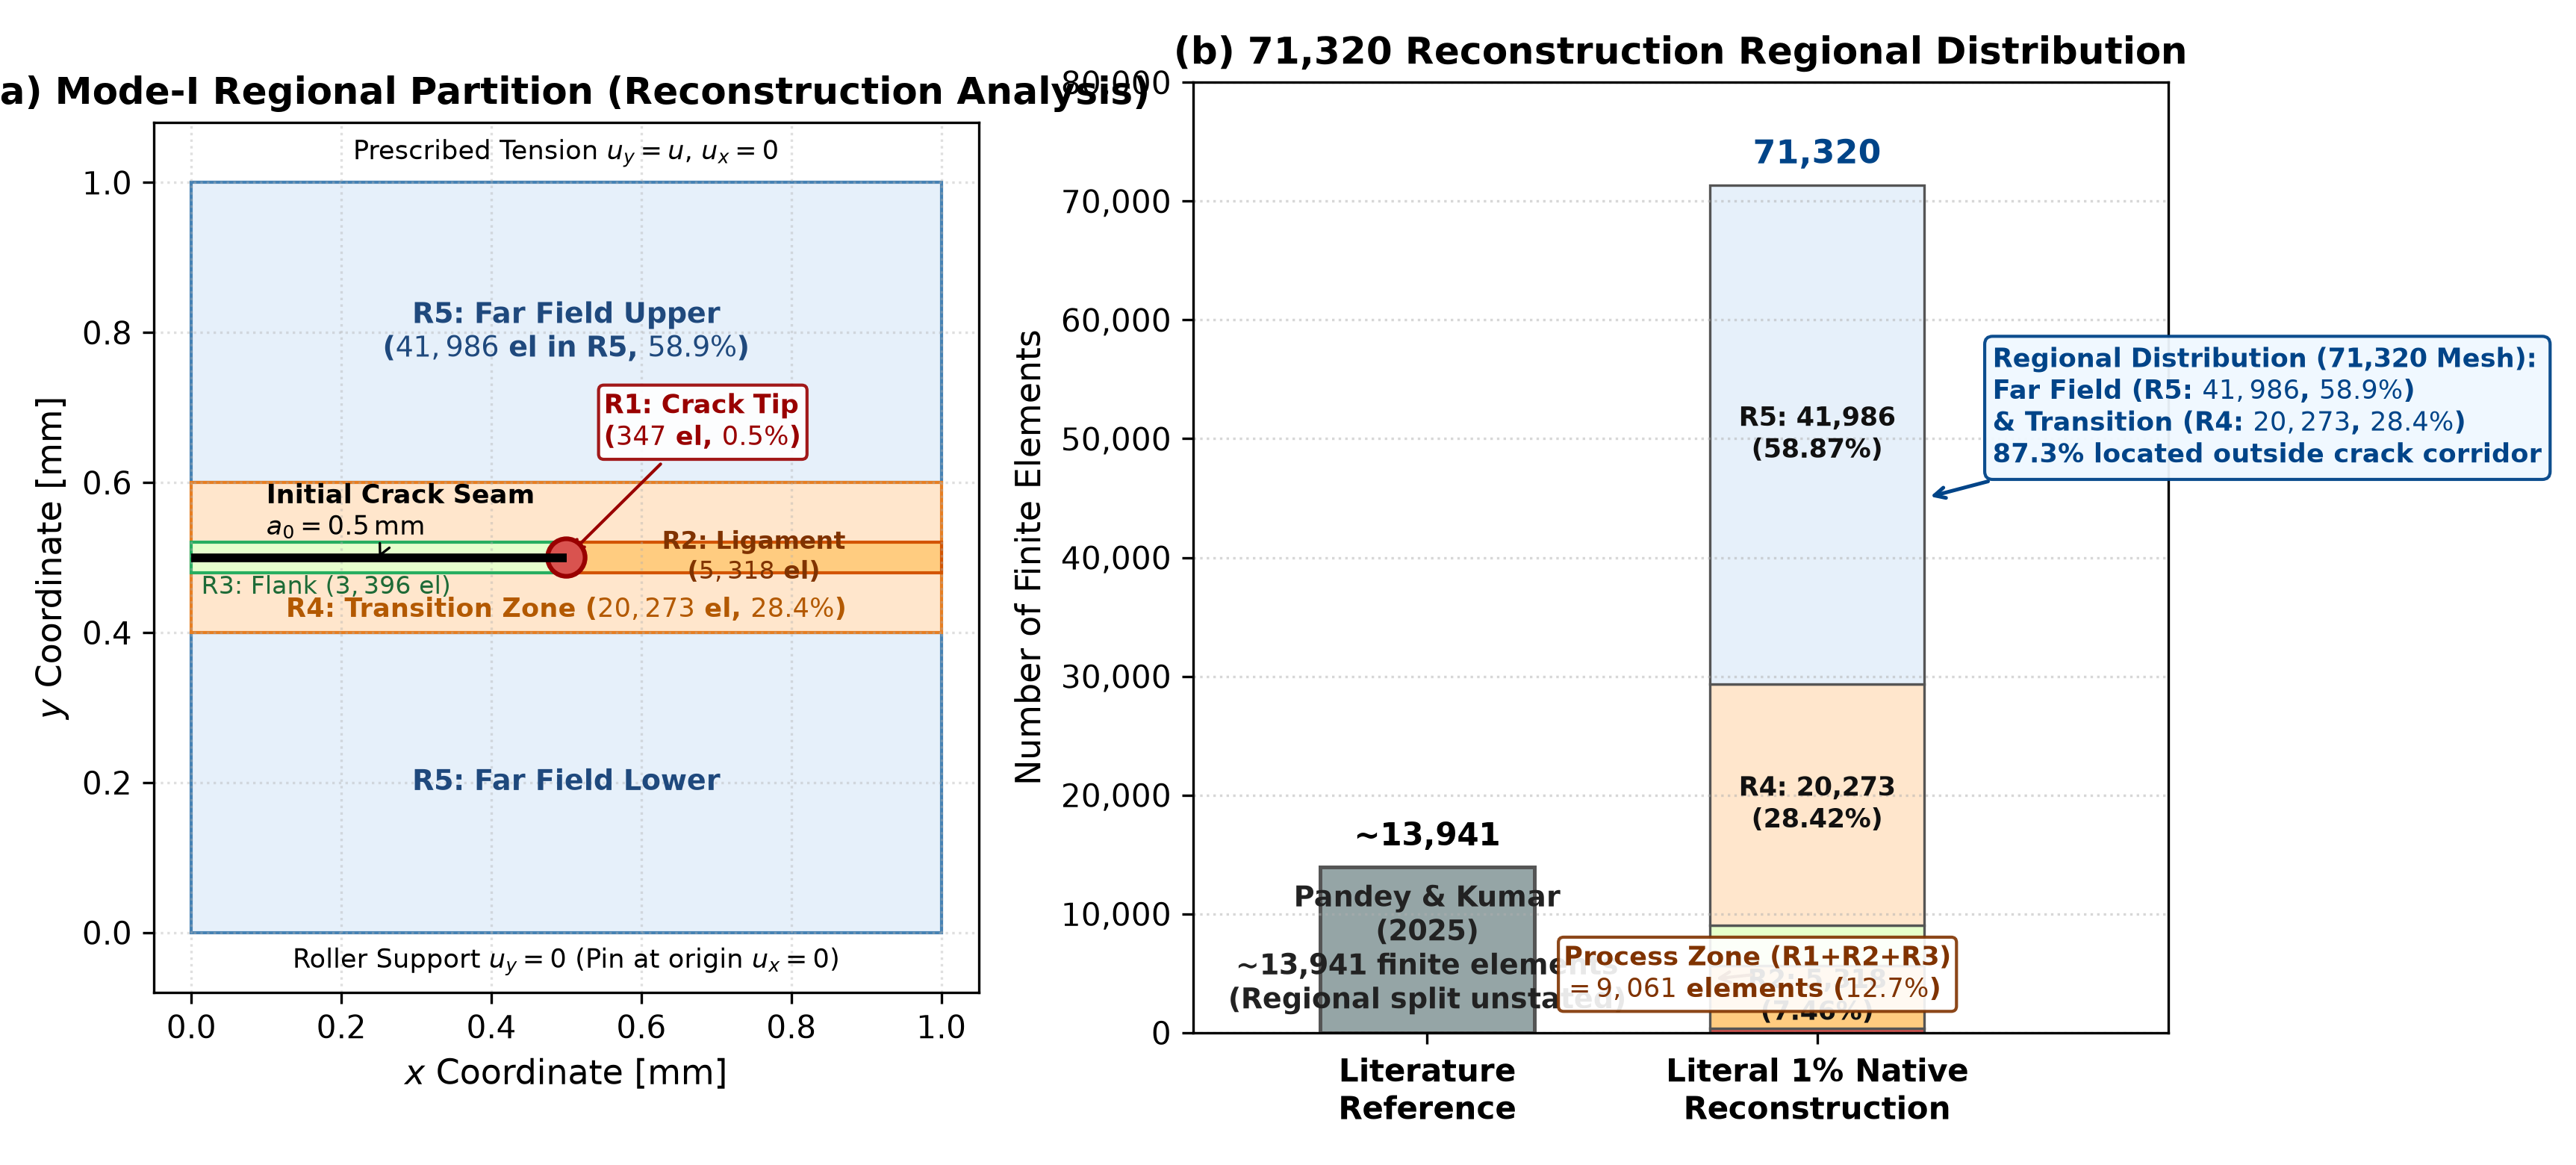
\includegraphics[width=0.82\textwidth]{fig2_gate5_mesh_discrepancy_and_regions.png}
  \caption{Mandatory Figure 2: Gate-5 mesh discrepancy audit. (a) Regional partition of the specimen used to analyze element placement in our $71{,}320$-element reconstruction. (b) Regional element count breakdown of our $71{,}320$-element reconstruction: the crack-tip process zone (R1+R2+R3) contains $9{,}061$ elements ($12.7\%$), while Far Field R5 ($41{,}986$ elements) and Transition R4 ($20{,}273$ elements) account for $87.3\%$ ($62{,}259$ elements) of the total mesh. Published literature reports $\approx 13{,}941$ total elements without a regional breakdown.}
  \label{fig:mesh_discrepancy}
\end{figure}

\subsection{Spatial Anatomy of the Discrepancy (Figure 2)}
Figure~\ref{fig:mesh_discrepancy} provides the spatial distribution for our publication-literal reconstruction of $71{,}320$ elements:
\begin{itemize}[leftmargin=4mm,itemsep=1pt,topsep=1pt]
  \item \textbf{Process Zone (R1 + R2 + R3):} Exactly $347$ crack-tip elements (R1), $5{,}318$ ligament elements (R2), and $3{,}396$ flank elements (R3), totaling \textbf{$9{,}061$ finite elements} ($12.7\%$ of the adapted mesh). This localized resolution is physically necessary to resolve the diffuse crack corridor with $h \le \ell_0 / 5$.
  \item \textbf{Far-Field and Transition (R4 + R5):} The transition zone (R4) contains $20{,}273$ elements ($28.4\%$) and the far field (R5) contains $41{,}986$ elements ($58.9\%$), totaling \textbf{$62{,}259$ finite elements ($87.3\%$) placed outside the crack corridor}.
\end{itemize}

\begin{quote}
\textbf{Scientific Evaluation:} Under the literal whole-domain remeshing rule (\texttt{All\_elem}, $\texttt{errorTarget}=1.0$), Abaqus refines the elastic far-field to satisfy the $1.0\%$ relative stress error threshold. The accessible evidence does not identify which unpublished implementation detail accounts for the reported $\approx 13{,}941$-element mesh. Possible distinctions such as call-site parameter linkage or an unstated region definition remain hypotheses requiring author information; neither is established.
\end{quote}

\clearpage

\section{Epistemological Audit: Knowns, Verifications, and Open Questions}
\label{sec:epistemological_audit}

\subsection{Claims Discipline and Epistemological Categorization}
To maintain the highest scientific rigor, every finding in this Master's thesis is strictly separated into three epistemic tiers:
\begin{enumerate}[label=\textbf{Tier \arabic*:},leftmargin=18mm,itemsep=0.5pt,topsep=1pt]
  \item \textbf{I Know This:} Analytical definitions, benchmark geometry, constitutive constants, and published literal text.
  \item \textbf{I Verified This Numerically:} Empirical results demonstrated by exact solver runs, output database extractions, and SHA-256 checksums.
  \item \textbf{I Do Not Yet Know This:} Genuine scientific open questions arising from omitted publication details or software internals.
\end{enumerate}

\begin{table}[htbp]
  \centering
  \scriptsize
  \renewcommand{\arraystretch}{1.08}
  \caption{Comprehensive epistemological audit table for the Mode-I adaptive remeshing reproduction.}
  \label{tab:epistemological_matrix}
  \begin{tabularx}{\textwidth}{L{52mm} L{42mm} L{48mm}}
    \toprule
    \textbf{Scientific Statement / Feature} & \textbf{Epistemic Status} & \textbf{Empirical Evidence / Basis} \\
    \midrule
    Plate geometry ($1\times 1\,\mathrm{mm}$) and sharp crack seam ($a_0 = 0.5\,\mathrm{mm}$, $y=0.5\,\mathrm{mm}$) & \textbf{I know this from theory \& definition} & Benchmark specification; zero-gap slit seam representation. \\
    \addlinespace
    Elastic constants ($E=210\,\mathrm{GPa}, \nu=0.3$) and fracture parameters ($G_c=2.7\,\mathrm{N/mm}, \ell_0=7.5\,\mu\mathrm{m}$) & \textbf{I know this from the publication} & Pandey \& Kumar \citep{Pandey2025}, Section~4.1; Table~1. \\
    \addlinespace
    RemeshingRule parameters (\texttt{MISESERI}, $\texttt{errorTarget}=1.0$, $h_{\min}=0.001$, $h_{\max}=0.020$) & \textbf{I know this from the publication} & Pandey \& Kumar \citep{Pandey2025}, Listing~1 (hard-coded parameters). \\
    \addlinespace
    Fixed-mesh reference reproduces literature ($F_{\max}=0.7578\,\mathrm{kN}$, $u=5.86\,\mu\mathrm{m}$, $K_0=137.95\,\mathrm{kN/mm}$) & \textbf{I verified this numerically} & Job \texttt{1398090}; $15{,}192$ elements; $-0.029\%$ error vs literature anchor. \\
    \addlinespace
    Canonical Mode-I pre-analysis consists of $2{,}906$ elements and $2{,}906$ \texttt{WHOLE\_ELEMENT} errors & \textbf{I verified this numerically} & \texttt{JOB1\_LOAD\_1p0X.odb} field extraction; retired old $3{,}930$-row dataset. \\
    \addlinespace
    Abaqus \texttt{pre} enforces $\le 16$ entries per line in free-format \texttt{*NSET} without \texttt{GENERATE} & \textbf{I verified this numerically} & Job \texttt{1404318} parser limit test; Abaqus documentation \citep{Abaqus2023}. \\
    \addlinespace
    Stiffness anomaly was caused by \texttt{*NSET} 16-entry limit where Abaqus issued preprocessing warnings and retained only 16 of 150 \texttt{N\_BOTTOM} nodes & \textbf{I verified the causal mechanism} & Verified \texttt{.dat} warnings; bottom-edge lift up to $\approx 48.34\%$ of stroke in malformed case vs $u_2=0$ in corrected case. \\
    \addlinespace
    Line wrapping ($\le 16$ items/line) recovers reference stiffness ($K_0=138.021\,\mathrm{kN/mm}$ frozen) & \textbf{I verified this numerically} & Job \texttt{1405044} (frozen); Job \texttt{1404933} (full fracture $K_0 \approx 137.821\,\mathrm{kN/mm}$). \\
    \addlinespace
    Solver asymmetry and companion elements do not affect structural stiffness ($0.000\%$ change) & \textbf{I verified this numerically} & Factorial runs 72b--79; formal retraction of asymmetry hypothesis. \\
    \addlinespace
    Literal 1\% remeshing generates $71{,}320$ elements identically across Abaqus 2019--2023 & \textbf{I verified this numerically} & Four-generation Linux release audit (Abaqus 2019, 2021, 2022, 2023 identical). \\
    \addlinespace
    Process zone contains $9{,}061$ elements; far-field and transition account for $62{,}259$ elements ($87.3\%$) of our reconstruction & \textbf{I verified this numerically} & 5-region spatial decomposition of 71,320-element mesh (Figure~\ref{fig:mesh_discrepancy}). \\
    \addlinespace
    Which unpublished implementation detail accounts for the reported $\approx 13{,}941$-element mesh & \textbf{I do not yet know this} & Accessible evidence does not identify unpublished settings (e.g. region definition or call-site linkage); hypotheses unestablished without author input. \\
    \bottomrule
  \end{tabularx}
\end{table}

\begin{quote}
\textbf{Epistemological Principle:} Stating \emph{``I do not yet know this''} is scientifically superior to advancing an unsupported hypothesis. The thesis maintains absolute fidelity to demonstrated numerical evidence.
\end{quote}

\clearpage

\section{Supervisor Decisions Required \& Action Paths}
\label{sec:supervisor_decisions}

\subsection{Decision Context for the 17 September 2026 Meeting}
With the complete resolution of the stiffness anomaly (Priority Question A is \textbf{\texttt{RESOLVED\_AND\_CLOSED}}), the simulation demonstrates excellent mechanical fidelity to the benchmark reference ($K_0$ within $0.09\%$, $F_{\max}$ within $1.64\%$). 

The sole unresolved item in the Mode-I benchmark is Priority Question B (the $71{,}320$ vs $\approx 13{,}941$ finite element count discrepancy). An exhaustive 15-factor audit has proved that this discrepancy cannot be resolved through any accessible Abaqus parameter without departing from the published text.

\subsection{The Two Actionable Supervisor Decision Pathways}
The supervisor is requested to select one of two clear pathways to conclude Gate~5:

\begin{tcolorbox}[colback=blue!4!white,colframe=blue!75!black,title=\textbf{Option A: Accept Gate 5 as Externally Under-Specified \& Proceed with Mode-I Synthesis},top=1.5pt,bottom=1.5pt,left=3pt,right=3pt]
\textbf{Decision Description:}
\begin{itemize}[leftmargin=4mm,itemsep=0.5pt,topsep=1pt]
  \item Accept Gate~5 as externally under-specified based on the exhaustive 15-factor audit.
  \item Retain $71{,}320$ finite elements as the verified publication-literal reconstruction under $\texttt{errorTarget}=1.0$ and whole-specimen remeshing.
  \item Document $\approx 13{,}941$ as unresolved due to missing publication information.
  \item Proceed only with Mode-I thesis synthesis/documentation pending further supervisor direction.
\end{itemize}
\textbf{Scope Limitation:} Gate~7 (ABAQUSER), Mode-II benchmarks, state transfer, and higher-complexity work remain explicitly \textbf{ON HOLD} pending separate supervisor authorization.
\end{tcolorbox}

\vspace{0.2em}

\begin{tcolorbox}[colback=orange!4!white,colframe=orange!85!black,title=\textbf{Option B: Authorize Transmission of Author Reproducibility Inquiry},top=1.5pt,bottom=1.5pt,left=3pt,right=3pt]
\textbf{Decision Description:}
\begin{itemize}[leftmargin=4mm,itemsep=0.5pt,topsep=1pt]
  \item Approve sending the finalized 6-question reproducibility inquiry to the corresponding authors (Dr.~Anshul Pandey and Dr.~Sachin Kumar).
  \item Keep Gate~5 open pending the author response.
  \item No further target-tuning exercises are authorized; $\texttt{errorTarget}=1.0$ remains the publication-literal reference and numerical proximity at $2\%$ is not evidence of parameter identity.
\end{itemize}
\textbf{Scope Limitation:} Gate~7 (ABAQUSER), Mode-II benchmarks, state transfer, and higher-complexity work remain explicitly \textbf{ON HOLD} pending separate supervisor authorization.
\end{tcolorbox}

\begin{quote}
\textbf{Strict Governance Rule:} In strict accordance with supervisor safety guidelines, the prepared author inquiry remains \textbf{UNSENT} and will not be transmitted without explicit written authorization from the supervisor. Under both options, increasing model complexity remains prohibited until authorized.
\end{quote}

\subsection{Summary of Prepared Author Questions (Held Unsent)}
The prepared inquiry focuses exclusively on the missing reproducibility facts:
\begin{enumerate}[leftmargin=4mm,itemsep=0.5pt,topsep=1pt]
  \item \textbf{Remeshing Region Set:} Was \texttt{RemeshingRule} applied to the whole plate (\texttt{All\_elem}) or a local geometric corridor?
  \item \textbf{Exact Error Target:} Was $\texttt{errorTarget}=1.0$ applied without modification for the $\approx 13{,}941$ mesh?
  \item \textbf{Pre-Analysis Coarse Mesh:} What was the exact element and node count of the initial pre-analysis mesh?
  \item \textbf{Coarsening Settings:} Was \texttt{coarseningFactor} kept at \texttt{NOT\_ALLOWED} or enabled?
  \item \textbf{Abaqus Release:} Under which Abaqus version was the remeshing script executed?
  \item \textbf{Sizing Controls:} Were any additional mesh controls (e.g., \texttt{sizeDeviationFactor}) applied?
\end{enumerate}

\clearpage

\section{Technical Provenance Ledger \& References}
\label{sec:provenance_and_references}

\subsection{Authoritative Simulation Jobs and Telemetry Ledger}
All numerical results reported in this document are derived from exact solver jobs executed on the High-Performance Computing Cluster of TU Bergakademie Freiberg (\texttt{normal\_imfdfkmq} partition).

\begin{table}[htbp]
  \centering
  \scriptsize
  \caption{Technical provenance ledger of authoritative Mode-I simulation jobs.}
  \label{tab:provenance_ledger}
  \begin{tabularx}{\textwidth}{L{22mm} L{22mm} C{16mm} C{18mm} C{13mm} L{46mm}}
    \toprule
    \textbf{Job Identifier} & \textbf{Model Role} & \textbf{Abaqus} & \textbf{CPUs / Threads} & \textbf{Walltime} & \textbf{Primary Telemetry / Status} \\
    \midrule
    \texttt{1398090.mmaster02} & Fixed Ref Anchor & 2023.HF4 & 1 CPU (serial) & 06:31:00 & $F_{\max}=0.757778\,\mathrm{kN}$, $K_0=137.946\,\mathrm{kN/mm}$ \\
    \texttt{1399632.mmaster02} & DEFECTIVE PREPROC. (Diag.) & 2023.HF4 & 1 CPU (serial) & 35:08:00 & DEFECTIVE N\_BOTTOM (16/150 boundary nodes parsed); $K_0=122.38\,\mathrm{kN/mm}$ \\
    \texttt{1404312.mmaster02} & Boundary ODB Audit & 2023.HF4 & 1 CPU (serial) & 00:03:12 & Bitwise proof of 16-node card truncation \\
    \texttt{1404318.mmaster02} & Parser Limit Test & 2023.HF4 & 1 CPU (serial) & 00:01:24 & General 16-entry \texttt{*NSET} limit verified \\
    \texttt{1405044.mmaster02} & Corrected Frozen & 2023.HF4 & 1 CPU (serial) & 00:04:36 & $K_0 = 138.021\,\mathrm{kN/mm}$, 150/150 nodes, 0 lift \\
    \texttt{1404933.mmaster02} & Corrected Nom 1\% & 2023.HF4 & 1 CPU (serial) & 18:34:50 & $F_{\max}=0.745325\,\mathrm{kN}$, $K_0 \approx 137.821\,\mathrm{kN/mm}$ ($137.820804\,\mathrm{kN/mm}$) \\
    \texttt{1405003.mmaster02} & 4T Parity Twin & 2023.HF4 & 1 MPI $\times$ 4T & 05:42:15 & Stage-A parity verified; repeat pending \\
    \texttt{Abaqus 2019 GA} & 2019 Release Control & 2019 GA & 1 CPU (serial) & 00:05:10 & $71{,}320$ elements bitwise identical \\
    \texttt{1404968.mmaster02} & 2021 Release Control & 2021.HF26 & 1 CPU (serial) & 00:04:45 & $71{,}320$ elements bitwise identical \\
    \texttt{1404373.mmaster02} & 2022/2023 Controls & 2022/23 & 1 CPU (serial) & 00:04:30 & $71{,}320$ elements bitwise identical \\
    \texttt{1405055.mmaster02} & Top $u_1 = \mathrm{Free}$ & 2023.HF4 & 1 CPU (serial) & 00:04:15 & $55{,}761$ elements ($-21.8\%$) \\
    \texttt{1405056.mmaster02} & Reduced \texttt{CPE4R} & 2023.HF4 & 1 CPU (serial) & 00:06:10 & $103{,}706$ elements ($+45.4\%$) \\
    \bottomrule
  \end{tabularx}
\end{table}

\vspace{-0.5em}

\subsection{Cryptographic Checksums (SHA-256) \& Execution Commands}
{\scriptsize
\begin{itemize}[leftmargin=4mm,itemsep=0.5pt,topsep=1pt]
  \item User subroutine \texttt{f42\_mixed\_uel.for}: \texttt{4271c66804e82df4b03692ea407c9197825d19488a0fc438efab28a2a537f51a}
  \item Fixed reference input deck (\texttt{fixture\_h0015.inp}): \texttt{9f3b52dca622a57eb0155b55e3474fc3108c90ebdb52c253dd658d51d9ad2a71}
  \item Reconstructed nominal 1\% input deck (\texttt{PK\_M1\_NOM1.inp}): \texttt{6385a4a49c4fa66c6b3e77f0a8276f7a62bc61e138a0a9d19451dcf878bb71ef}
  \item Reference reaction force curve (\texttt{curve\_standard\_1398090.csv}): \texttt{780d05d39532e778802cdd8503cdd0df25568e412c3d4a51c50f4e001febede6}
  \item Corrected nominal 1\% curve (\texttt{curve\_1404933\_extracted.csv}): \texttt{f71f01d150b12355f7a9f4a4a19563fe6e046ec31d94fe5abe85c103eadf3d56}
\end{itemize}
}

\vspace{-0.4em}
{\footnotesize\textbf{Standard Abaqus CLI Reproduction Commands:}}
\begin{verbatim}
abaqus job=PK_M1_PRE input=PK_M1_PRE_CMS0020.inp interactive
abaqus cae noGUI=run_adaptive_remesh_canonical.py -- job=PK_M1_PRE
abaqus job=PK_M1_NOM1_STRICT input=PK_M1_NOM1_STRICT.inp \
       user=f42_mixed_uel.for cpus=1 interactive
\end{verbatim}

\vspace{-0.8em}
\renewcommand{\refname}{\normalsize References}
\setlength{\bibsep}{1.5pt}
\bibliographystyle{abbrvnat}
\bibliography{literature}


\end{document}
